% -*- latex -*-

%\documentclass[pdf,ps2pdf,12pt,report,strict]{SANDreport}
\documentclass[12pt,report,strict]{SANDreport}
\usepackage{pslatex}
\usepackage[fancyhdr]{latex2man}
\usepackage{ifthen}
\usepackage{xspace}
\usepackage{fancyvrb}

% Uncomment this if not a draft.
\usepackage[all,light]{draftcopy}

\usepackage{color}
\definecolor{yellow}{rgb}{1,1,0}
\definecolor{black}{rgb}{0,0,0}
\definecolor{ltcyan}{rgb}{.75,1,1}
\definecolor{red}{rgb}{1,0,0}

% This wonderful package allows hyphenation in tt fonts and hyphenation of
% words with underscores in them.
\usepackage[htt]{hyphenat}

\usepackage{makeidx}
\makeindex

\usepackage{hyperref}
\hypersetup{pdftitle={@TITLE@}}
\hypersetup{pdfauthor={Kenneth Moreland}}
% \hypersetup{colorlinks}
% \hypersetup{linkcolor=blue}
% \hypersetup{linkcolor=blue}
\hypersetup{breaklinks}
\hypersetup{pagebackref}
\hypersetup{pdfstartpage=3}

% -----------------------------------------------------------------------------
%
% Set the title, author, and date
%

\title{@TITLE@}
\author{Kenneth~Moreland \\
  Data Analysis and Visualization \\
  Sandia National Laboratories \\
  P.O. Box 5800  MS 0822 \\
  Albuquerque, NM  87185-0822 \\
  kmorel@sandia.gov
}

% There is a "Printed" date on the title page of a SAND report, so
% the generic \date should generally be empty.
\date{}

% -----------------------------------------------------------------------------
% Set some things we need for SAND reports. These are mandatory
%
\SANDnum{SAND2008-6739P}
\SANDprintDate{XXX 2008}
\SANDauthor{Kenneth~Moreland, Sandia}

% -----------------------------------------------------------------------------
% Include the markings required for the SAND report.  These are actually
% the default and not strictly necessary.
\SANDreleaseType{Unlimited Release}
\SANDmarkCover{Approved for public release; further dissemination unlimited.}

%-----------------------------------------------------------------------------
% The following definition does not have a default value and will not
% print anything, if not defined
%\SANDsupersed{SAND1901-0001}{January 1901}

%-----------------------------------------------------------------------------
% Commands for inserting common words.
\newcommand{\IceT}{IceT\xspace}
\newcommand{\OpenGL}{\index{OpenGL}OpenGL\xspace}
\newcommand{\MPI}{\index{MPI}{MPI}\xspace}

% Commands for words with special meanings.
\newcommand*{\keyterm}[1]{\textbf{#1}}

\newcommand{\sticky}[1]{{\color{red}\textsc{[#1]}}}

\CustomVerbatimEnvironment{code}{Verbatim}{fontsize=\small}
\newcommand*{\codeinput}[2][]{%
  \VerbatimInput[fontsize=\small,#1]{#2}%
}

% A special section for man pages.  We don't really want these to show up
% in the table of contents.
% \newcommand{\mansection}[1]{
%   \\[\baselineskip]
%   \textbf{\textsc{\large #1}} \\[0.5\baselineskip]
% }
\makeatletter
\renewcommand{\subsection}{\@startsection
  {subsection}
  {2}
  {0mm}
  {-\baselineskip}
  {0.5\baselineskip}
  {\normalfont\large\bfseries\scshape}
}
\makeatother
\newcommand*{\mansection}[1]{\subsection*{#1}}  

% The latex2man Name environment does not mesh well with the SAND
% environment, nor is it designed to have several man pages in the same
% document.  Thus, we change it to fit.
\newcommand*{\currentmansection}{none}
\renewenvironment{Name}[5]{
  % #1 Man Chapter
  % #2 Name
  % #3 Author
  % #4 Tool
  % #5 Title
  \clearpage
  \renewcommand{\currentmansection}{#2}
  \index{\currentmansection|(textbf}
  \lhead[#2]{}
  \rhead[]{#2}
  \phantomsection
  \addcontentsline{toc}{section}{\currentmansection}
  \label{manpage:#2}
  \mansection{Name}
  #5
}{
  \index{\currentmansection|)}
}

% Commands for typesetting C identifiers.
\newcommand{\textC}[1]{\texttt{#1}}                     % Basic C code.
\newcommand{\textCF}[1]{\textbf{\textC{#1}}}
\newcommand{\textCT}[1]{\textbf{\textC{#1}}}

\newcommand{\CType}[1]{\index{#1}\textCT{#1}}           % A documented type.
\newcommand{\CFunc}[2][!*!]{%                           % A documented function.
  % Only reference if not in that man section.
  \ifthenelse%
      {\equal{#1}{!*!}}%
      {\ifthenelse%
        {\equal{#2}{\currentmansection}}%
        {\textCF{#2}}%
        {\index{#2}\hyperref[manpage:#2]{\textCF{#2}}}%
      }%
      {\ifthenelse%
        {\equal{#1}{\currentmansection}}%
        {\textCF{#2}}%
        {\index{#1}\hyperref[manpage:#1]{\textCF{#2}}}%
      }%
}
\newcommand*{\CFuncExternal}[1]{%                       % An external function.
  \index{#1}%
  \textCF{#1}%
}
\newcommand*{\CFuncSeeAlso}[1]{%                        % A see also reference.
  \hyperref[manpage:#1]{\textCF{#1}}%
}
\newcommand*{\CTypeExternal}[1]{\CType{#1}}             % An external type.

\newcommand*{\CArg}[1]{\emph{\textC{#1}}}               % A function argument.
\newcommand*{\CEnum}[1]{\index{#1}\textbf{\textC{#1}}}  % A const enumeration.
\newcommand*{\CErrorEnum}[1]{\textbf{\textC{#1}}}       % An error constant.

% Functions that have aliases for cross referencing and indexing.
\newcommand{\icetBoundingBoxf}{\CFunc[icetBoundingBox]{icetBoundingBoxf}\xspace}
\newcommand{\icetBoundingBoxd}{\CFunc[icetBoundingBox]{icetBoundingBoxd}\xspace}
\newcommand{\icetEnable}{\CFunc[icetEnable]{icetEnable}\xspace}
\newcommand{\icetDisable}{\CFunc[icetEnable]{icetDisable}\xspace}
\newcommand{\icetGetBooleanv}{\CFunc[icetGet]{icetGetBooleanv}\xspace}
\newcommand{\icetGetDoublev}{\CFunc[icetGet]{icetGetDoublev}\xspace}
\newcommand{\icetGetFloatv}{\CFunc[icetGet]{icetGetFloatv}\xspace}
\newcommand{\icetGetIntegerv}{\CFunc[icetGet]{icetGetIntegerv}\xspace}
\newcommand{\icetGetPointerv}{\CFunc[icetGet]{icetGetPointerv}\xspace}
\newcommand{\icetGetColorBuffer}{\CFunc{icetGetColorBuffer}\xspace}
\newcommand{\icetGetDepthBuffer}{%
  \ifthenelse%
    {\equal{\currentmansection}{icetGetColorBuffer}}%
    {\CFunc[icetGetColorBuffer]{icetGetDepthBuffer}}%
    {\CFunc{icetGetDepthBuffer}}%
    \xspace%
}

%-----------------------------------------------------------------------------
% The actual document.

\begin{document}

\sloppy
\maketitle

% An abstract is required for SAND reports.

\begin{abstract}
  The Image Composition Engine for Tiles (\IceT) is a high-performance
  sort-last parallel rendering library.  In addition to providing
  accelerated rendering for a standard display, \IceT provides the unique
  ability to generate images for tiled displays.  The overall resolution of
  the display may be several times larger than any viewport that may be
  rendered by a single machine.  This document is an overview of the user
  interface to \IceT.
\end{abstract}

%-----------------------------------------------------------------------------
% In case we every need an acknowledgement section.
\clearpage
\chapter*{Acknowledgement}

I would like to thank Brian Wylie.  It was his ``big ideas'' that got the
ball rolling on the \IceT algorithms and library, and it was his continuing
vision that pushed us on this path to parallel rendering.

I would also like to thank the folks at Kitware, Inc. for adopting the
\IceT library as the parallel rendering library for ParaView.  They also
maintain the \IceT code repository.  Without them, \IceT would probably be
collecting dust on a crashed RAID somewhere.

% -----------------------------------------------------------------------------
% The table of contents and list of figures and tables
% Comment out \listoffigures and \listoftables if there are no
% figures or tables. Make sure this starts on an odd numbered page
\cleardoublepage                % TOC needs to start on an odd page
\tableofcontents
\listoffigures
% \listoftables

% -----------------------------------------------------------------------------
% This is where the body of the report begins.
\SANDmain       % Start the main part of the report.

% -*- latex -*-


\chapter{Introduction}
\label{chap:Introduction}

The Image Composition Engine for Tiles (\IceT) is an API designed to enable
OpenGL applications to perform Sort-Last parallel rendering on very large
displays.  The displays are assumed to be tile displays.  The overall
resolution of the display may be several times larger than any viewport
that may be rendered by a single machine.  It is also assumed that several
processes in the parallel application are
\index{display~process}\keyterm{display processes}.  That is, their entire
display window makes up part of the display.

The design philosophy behind \IceT is to allow very large sets of polygons
to be displayed on very high resolution displays.  As such, fast frame
rates are sacrificed in lieu of very scalable and very high polygon/second
rendering rates.  That said, there are many features in \IceT that allow an
application to achieve interactive rates.  These include image inflation,
floating viewports, active pixel encoding, and data replication.  Together,
these features make \IceT a versatile parallel rendering application that
provides near optimal parallel rendering under most data size and image
size combinations.  As an example, the ParaView
application\footnote{\href{http://www.paraview.org}{http://www.paraview.org}}
is using \IceT for all of its parallel rendering needs ranging from a
desktop sized image to the world's largest tile displays and from polygon
counts ranging from 1 to 1 million (and growing).

\IceT is designed to take advantage of
\index{spatial~decomposition}\keyterm{spatial decomposition} of the
geometry being rendered.  That is, it works best if all the geometry on
each process is located in as small a region of space as possible.  When
this is true, each process usually projects geometry on only a small
section of the screen.  This results in less work for the compositing
engine.  This is of particular importance for displays with a large number
of pixels.

\IceT can also be used to perform sort-last parallel rendering to a single
display.  Such \index{single-tile~rendering}\keyterm{single-tile rendering}
is simply a special case of the multi-tile display \IceT was designed for.
Many of the optimizations done by \IceT apply to the single-tile mode.
Using \IceT for this purpose is quite worthwhile.  \IceT's performance
should rival that of other such software image compositors.

The rest of this document describes the use of the
\IceT
API.  There are also separate manual pages for each of the functions
described here.  For more details on
\IceT's
algorithms, see:

\begin{quote}
  Moreland, Wylie, and Pavlakos.  ``Sort-last parallel rendering for
  viewing extremely large data sets on tile displays,'' In
  \emph{Proceedings of IEEE Symposium on Parallel and Large-Data
    Visualization and Graphics}, October 2001, pp. 85--154.
\end{quote}


\section{A Parallel Rendering Primer}
\label{sec:Introduction:Parallel_Rendering_Primer}

\IceT requires you to know very little about parallel rendering and their
algorithms.  However, it is helpful to know the basic idea behind \IceT's
algorithms.  This section gives a brief introduction to how \IceT renders
in parallel.

Parallel rendering algorithms are classified as
\index{sort-first}\keyterm{sort-first},
\index{sort-middle}\keyterm{sort-middle}, or
\index{sort-last}\keyterm{sort-last}.  The key distinguishing feature of
each class is how primitives are distributed amongst processes.  As
demonstrated in Figure~\ref{fig:Introduction:ParallelRenderingClasses},
sort-first and sort-middle algorithms allocate screen space to processes
and send the appropriate geometry to each process every frame whereas
sort-last algorithms render static partitions of geometry in each process
and then composite the resulting images to a single image.\footnote{In the
  interest of brevity and clarity, I am intentionally leaving out details
  that are unimportant to understanding \IceT such as hybrid algorithms and
  differences between sort-first and sort-middle algorithms.}  \IceT is a
sort-last parallel rendering library.

\begin{figure}
  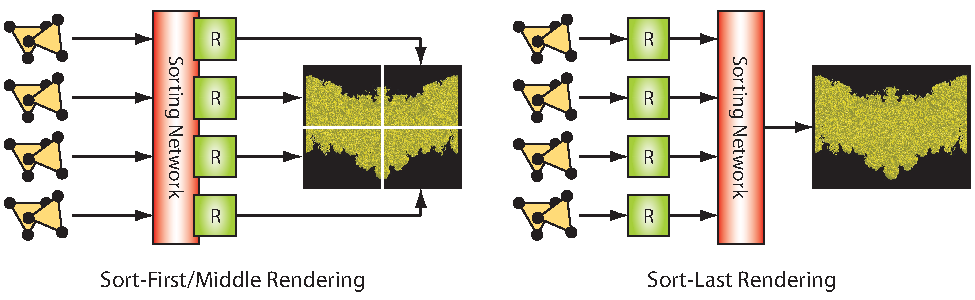
\includegraphics{images/ParallelRenderingClasses}
  \label{fig:Introduction:ParallelRenderingClasses}
  \caption{The differences between parallel rendering classes.  Sort-first
    and sort-middle algorithms transfer geometric data.  Sort-last
    algorithms transfer image data.}
\end{figure}

A convenient feature of sort-last rendering is that an application needs to
change very little about how it renders geometry.  The geometry is rendered
the same in parallel as it is in serial; the only difference is that each
process only renders a subset of the geometry.  The typical operation of a
parallel application using sort-last rendering is to simply render locally
and then composite the images.

When rendering to a tiled display, as \IceT allows you to do, there is an
added level of complexity introduced because the graphics system is often
not capable of rendering an image large enough for the entire display.
Thus, image compositing for a tiled display requires a loop that can
iteratively render images for each tile and composite them.  \IceT handles
this looping and interfaces with the rendering functions of your
application through a callback mechanism.  This will be described in the
following chapters.


% -*- latex -*-

\chapter{Tutorial}
\label{chap:Tutorial}

In this chapter we outline the steps required to create a simple \IceT
application from building the \IceT source, using the created libraries,
and writing your own applications.  \IceT is solely responsible for the
image composition part of parallel rendering.  Thus, it relies on separate
systems for rendering and communication.  The two most common libraries
for these features are \index{OpenGL}\keyterm{OpenGL} and
\index{MPI}\keyterm{MPI} (the Message Passing Interface), respectively.
\IceT has support libraries for directly using these two systems and we
will use them for this tutorial.

This tutorial assumes the reader is familiar with \OpenGL or some similar
rendering system.  If this is your first experience with \OpenGL programing,
consider trying some typical serial rendering before jumping into the
parallel rendering domain.  A familiarity with \MPI is also helpful.

\section{Building \IceT}
\label{sec:Tutorial:Building_IceT}

The \IceT build process is very portable.  It is regularly compiled on
Microsoft Windows, Macintosh OS X, and a wide variety of Unix
implementations.  \IceT can be built with any \index{OpenGL}OpenGL~1.1
compliant installation.  Most modern operating systems come distributed
with \OpenGL.  For those that are not, you can usually use the
\index{Mesa~3D}\keyterm{Mesa 3D} library
(\href{www.mesa3d.org}{www.mesa3d.org}), a software implementation of
\OpenGL.  An installation of \MPI is also almost always needed, although
not strictly required.  \index{OpenMPI}\keyterm{OpenMPI}
(\href{http://www.open-mpi.org/}{http://www.open-mpi.org/}) and
\index{MPICH}\keyterm{MPICH}
(\href{http://www.mcs.anl.gov/mpi/mpich2/}{http://www.mcs.anl.gov/mpi/mpich2/})
are two free and widely portable implementation of \MPI.

\IceT uses \index{CMake}\keyterm{CMake} to build across so many different
platforms.  As such, you will have to download the CMake build tools from
\href{www.cmake.org}{www.cmake.org} and install.  Then, create a build
directory and run the CMake program (from the ``Start'' menu on Windows or
ccmake on Unix and Mac OS X).  CMake will determine the parameters of your
system and do its best to find libraries on which \IceT depends.  The CMake
program, shown in Figure~\ref{fig:Tutorial:ccmake} will also provide a GUI
to allow you to easily change build parameters and external libraries.
\begin{figure}
  \centering
  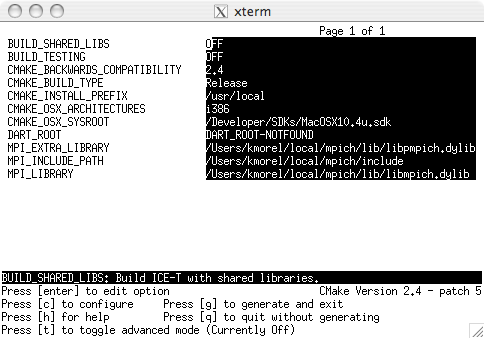
\includegraphics[height=1.5in]{images/ccmakeUnix}
  \qquad
  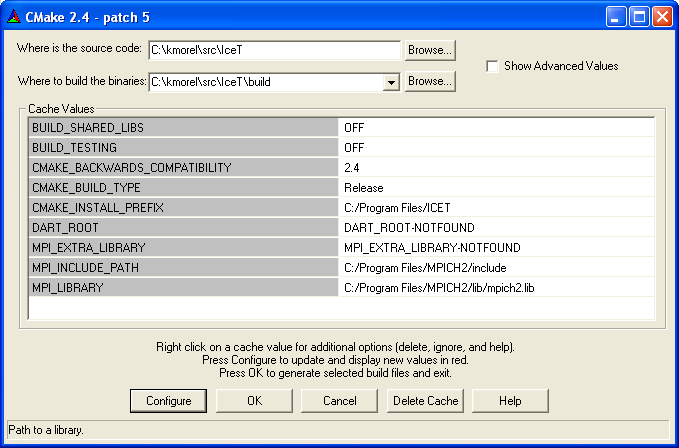
\includegraphics[height=1.5in]{images/ccmakeWindows}
  \caption[CMake user interface.]{The CMake user interface.  The Unix
    version is on the left whereas the Microsoft Windows version is on the
    right.}
  \label{fig:Tutorial:ccmake}
\end{figure}

CMake will generate a set of build files for the local system.  The type of
files depends on the type of machine you are using and the compile system
you have chosen to use.  On Unix machines, make files are the most common.
On Windows, you usually generate MSVC project files or nmake files.  On Mac
OS X, either make files or Xcode project files are commonly generated based
on user selection.  You then use the native build system to build and,
optionally, install \IceT.

\section{Linking to \IceT Libraries}
\label{sec:Tutorial:Linking_to_IceT_Libraries}

\IceT comes with three libraries:
\index{IceTCore (library)}\keyterm{IceTCore},
\index{IceTGL (library)}\keyterm{IceTGL}, and
\index{IceTMPI (library)}\keyterm{IceTMPI}.  The actual filenames of these
libraries varies depending on the filesystem and build type.  For example,
on most Unix systems, a static build results in filenames of
\index{libIceTCore.a}libIceTCore.a and the like whereas shared libraries
are \index{libIceTCore.so}libIceTCore.so.  Windows has libraries with names
like \index{IceTCore.lib}IceTCore.lib as well as
\index{IceTCore.dll}IceTCore.dll if building shared libraries.  However,
the difference in these filenames usually hidden by the build system,
especially if you use a portable build system like \index{CMake}CMake.

You are, of course, free to use whatever build system you like, whether it
be system specific or cross platform.  Using \IceT is simply a matter of
finding the header and library files.  However, because \IceT is built with
\index{CMake}CMake, it comes with some extra facilities for helping other
CMake builds find it.  This section will give you the bare minimum you need
to set up CMake to build an application using \IceT.  Readers interested in
learning more about CMake should pick up a copy of \emph{Mastering CMake}
by Ken Martin and Bill Hoffman.

You define a build system with CMake by creating a
\index{CMakeLists.txt}\keyterm{CMakeLists.txt} file.  The CMakeLists.txt
file is basically a simple script that gives commands to CMake to tell it
how to build your project.  Most CMakeLists.txt files start with the
\textC{PROJECT} command, which associates a name with your project and
optionally specifies a language.
\begin{code}
PROJECT(IceT_Tutorial)
\end{code}

To use \IceT from within your CMake project, run the
\index{FIND\_PACKAGE}\textC{FIND\_PACKAGE} command.  This command instructs
CMake to find the \index{IceTConfig.cmake}IceTConfig.cmake file, which is
written to \IceT's build or install directory and contains all the
necessary build settings.
\begin{code}
FIND_PACKAGE(IceT REQUIRED)

INCLUDE_DIRECTORIES(${ICET_INCLUDE_DIRECTORIES})
\end{code}
%$

Assuming that CMake finds \IceT, the CMake variable
\CEnum{ICET\_INCLUDE\_DIRS} is defined and can be passed to the
\index{INCLUDE\_DIRECTORIES}\textC{INCLUDE\_DIRECTORIES} CMake command.
The variables \CEnum{ICET\_CORE\_LIBS}, \CEnum{ICET\_GL\_LIBS}, and
\CEnum{ICET\_MPI\_LIBS} are also defined and can be used with a
\index{TARGET\_LINK\_LIBRARIES}TARGET\_LINK\_LIBRARIES command to link in
the respective \IceT libraries.

Any application using \IceT will probably also be using \OpenGL and \MPI.
In addition, the example in the following section also uses
\index{GLUT}GLUT for window management.  CMake comes with modules to find
all three of these libraries, which makes it easy to include in our
project.

\begin{code}
FIND_PACKAGE(OpenGL REQUIRED)
FIND_PACKAGE(GLUT REQUIRED)
FIND_PACKAGE(MPI REQUIRED)

MARK_AS_ADVANCED(CLEAR
  MPI_INCLUDE_PATH
  MPI_LIBRARY
  MPI_EXTRA_LIBRARY
  )

INCLUDE_DIRECTORIES(
  ${OPENGL_INCLUDE_DIR}
  ${MPI_INCLUDE_PATH}
  ${GLUT_INCLUDE_DIR}
  )
\end{code}
%$

The only thing left to do is to tell CMake to build a program from a set of
sources and libraries specified with the
\index{ADD\_EXECUTABLE}\textC{ADD\_EXECUTABLE} and
\index{TARGET\_LINK\_LIBRARIES}\textC{TARGET\_LINK\_LIBRARIES} commands,
respectively.
\begin{code}
ADD_EXECUTABLE(Tutorial Tutorial.c)
TARGET_LINK_LIBRARIES(Tutorial
  ${OPENGL_LIBRARIES}
  ${GLUT_LIBRARIES}
  ${MPI_LIBRARY}
  ${MPI_EXTRA_LIBRARY}
  ${ICET_CORE_LIBS}
  ${ICET_GL_LIBS}
  ${ICET_MPI_LIBS}
  )
\end{code}
%$

\section{Creating \IceT Enabled Applications}
\label{sec:Tutorial:Creating_IceT_Enabled_Applications}

To use \IceT, include its header: \index{IceT.h}\textC{IceT.h}.  If you are
using \OpenGL for rendering, you will probably also want to use \IceT's
\OpenGL integration functions in \index{IceTGL.h}\textC{IceTGL.h}.  You will
almost always need to also include the header containing an \MPI version of
an \IceT communicator: \index{IceTMPI.h}\textC{IceTMPI.h}.  On the rare
occasion that you need to use \IceT with a communication layer other than
\MPI, you can define a custom communicator as described in
Chapter~\ref{chap:Communicators}.
\begin{code}
#include <IceT.h>
#include <IceTGL.h>
#include <IceTMPI.h>
\end{code}

Before you call any \IceT functions, you need to initialize \MPI by calling
\textC{MPI\_Init}\index{MPI\_Init}.  You will also need to create an
\index{context!\OpenGL}\keyterm{\OpenGL context}.  In other words, you need
to make the rendering window in which the \OpenGL rendering commands will
go.  The process for doing this is greatly dependent on the windowing
system and beyond the scope of this document.  It is usually easiest to use
a third party API to do this.  If you are not already using a GUI tool that
generates \OpenGL windows for you, then the \index{GLUT}\keyterm{GLUT} API
is a popular choice for simple applications.

You will then need to initialize \IceT itself.  Do this by first creating
an \IceT \index{communicator}\keyterm{communicator} from an \MPI
communicator and then using that to create an
\index{context!\IceT}\keyterm{\IceT context}.  When using \OpenGL, you also
need to initialize the OpenGL-specific code in \IceT by calling
\CFunc{icetGLInitialize}.

\index{icetCreateMPICommunicator}
\index{icetCreateContext}
\begin{code}
comm = icetCreateMPICommunicator(MPI_COMM_WORLD);
context = icetCreateContext(comm);
icetGLInitialize();
\end{code}

In the proceeding code, \textC{comm} is of type
\index{IceTCommunicator}\textC{IceTCommunicator} and \textC{context} is of
type \index{IceTContext}\textC{IceTContext}.

Now that we have created and activated an \IceT communicator, as well as
initialized the \IceT \index{state}\keyterm{state}, we can start using
\IceT.  It is often useful to first query \IceT on the size of the parallel
job it is running in and what is the local process id, or
\index{rank}\keyterm{rank}.  The values are stored in variables of type
\index{IceTInt}\textC{IceTInt}.

\index{icetGet}
\index{ICET\_RANK}
\index{ICET\_NUM\_PROCESSES}
\begin{code}
icetGetIntegerv(ICET_RANK, &rank);
icetGetIntegerv(ICET_NUM_PROCESSES, &num_proc);
\end{code}

Before rendering, we need to tell \IceT the layout of the tiled display
using the \CFunc{icetResetTiles} and \CFunc{icetAddTile} functions.  These
commands must be executed with the same arguments on all processes of the
parallel job.  \IceT will assume that you setup the same display layout
everywhere.

If you are not actually driving a tiled display and instead just generating
a desktop-sized image, the following commands will correctly establish the
\IceT state (assuming \textC{WINDOW\_WIDTH} and \textC{WINDOW\_HEIGHT}
correctly reflect the desired image dimensions).

\begin{code}
icetResetTiles();
icetAddTile(0, 0, WINDOW_WIDTH, WINDOW_HEIGHT, 0);
\end{code}

The \CFunc{icetResetTiles} function simply tells \IceT that you are about
to define a display layout.  Each call to \CFunc{icetAddTile} defines a
tile in the display.  In the case of a single image, the
\index{single-tile~rendering}\keyterm{single-tile rendering} mode,
\CFunc{icetAddTile} is called only once.  The first two arguments to
\CFunc{icetAddTile} have no effect in this mode.  The third and fourth
arguments are the width and height of the image to create.  Usually you set
this to the width and the height of the display window, but the
\hyperref[sec:Customizing_Compositing:Image_Inflation]{Image Inflation}
section in Chapter~\ref{chap:Customizing_Compositing} describes other usage
for these parameters.  The final argument is the rank of the
\index{display~process}\keyterm{display process}.  After a rendering the
final complete image will available only on this process.  In the example
above, we have directed the image to go to process zero, often referred to
as the \index{root~process}\keyterm{root process}.

To define an actual tiled display, simply call the \CFunc{icetAddTile}
function multiple times.  When describing tiles in a display, the first two
arguments of \CFunc{icetAddTile} describe where the lower left corner of
the tile is located in respect to the overall display.  All together, the
first four arguments specify a viewport for the tile in an a single,
cohesive high resolution display (which is what we are trying to achieve
with our tiled display).  The code below defines a $2 \times 2$ tiled
display with the top two tiles displayed by processes 0 and 1 and the
bottom two tiles displayed by processes 2 and 3.
\begin{code}
icetResetTiles();
icetAddTile(0,           WINDOW_HEIGHT, WINDOW_WIDTH, WINDOW_HEIGHT, 0);
icetAddTile(WINDOW_WIDTH,WINDOW_HEIGHT, WINDOW_WIDTH, WINDOW_HEIGHT, 1);
icetAddTile(0,           0,             WINDOW_WIDTH, WINDOW_HEIGHT, 2);
icetAddTile(WINDOW_WIDTH,0,             WINDOW_WIDTH, WINDOW_HEIGHT, 3);
\end{code}

\IceT contains several \index{strategy}\keyterm{strategies} for image
composition.  Changing the strategy modifies the algorithm \IceT uses for
parallel image compositing.  You need to tell \IceT which strategy to use
with the \CFunc{icetStrategy} function.  The code below sets \IceT to use
the \index{strategy!reduce}\keyterm{reduce strategy}, which has proven to
be an all-around good performer.
\begin{code}
icetStrategy(ICET_STRATEGY_REDUCE);
\end{code}
However, when rendering only a single tile, your best bet is to use the
\index{strategy!sequential}\keyterm{sequential strategy}, which bypasses
some of the collective communication necessary for other strategies.
\begin{code}
icetStrategy(ICET_STRATEGY_SEQUENTIAL);
\end{code}
Chapter~\ref{chap:Strategies} gives more detailed descriptions and advice
about the strategies.  Like with the display set up, all processes must set
the same strategy.

\IceT is almost ready to go.  We just need to tell it some minimal
information about how to render your geometry.  First, \IceT needs to know
the spatial extent of the geometry to be drawn (in object space).  The most
natural way to do this is to use the \CFunc{icetBoundingBox} function,
which defines an axis-aligned box defined by the minimum and maximum
coordinates in each dimension.
\begin{code}
icetBoundingBoxf(x_min, x_max, y_min, y_max, z_min, z_max);
\end{code}
The parameters can, and should be, different on each process, since each
process will have a different partition of data.  Strictly speaking,
identifying the geometry bounds is not necessary.  If they are not defined,
\IceT will assume the geometry covers the entire screen.  When rendering a
single small image, the information is of little consequence.  However,
when rendering larger images this information can dramatically improve the
performance of image composting.  Specifying the bounds can be critical on
large tile displays.

The second and final piece of information \IceT needs is a way to draw your
geometry.  \IceT achieves this through a
\index{drawing~callback}\index{callback|see{drawing~callback}}\index{rendering~callback|see{drawing~callback}}\keyterm{drawing
  callback}.

\index{icetGLDrawCallback}
\begin{code}
icetGLDrawCallback(drawScene);
\end{code}

The drawing callback is a pointer to any function that issues \OpenGL
commands that render geometry to the active frame buffer.  The callback is
free to issue most \OpenGL commands so long as it restores all the \OpenGL
state (except, of course, frame buffer contents).  Also, the callback
function should modify neither the projection matrix nor the clear color.
Care needs to be taken if the callback modifies the model view matrix.
More details are given in the
\hyperref[sec:Basic_Usage::Drawing_Callback]{Drawing Callback} section of
Chapter~\ref{chap:Basic_Usage}.

\IceT is now ready to render.  Rendering is initiated with a call to
\CFunc{icetGLDrawFrame}.  The \CFunc{icetGLDrawFrame} must be called on all
processes.  The function will render the scene using the provided
\index{drawing~callback}drawing callback, composite the image, and place
the appropriate images in the back \OpenGL buffers of the appropriate
\index{display~process}display processes.
\begin{code}
icetGLDrawFrame();
\end{code}

Parallel rendering is now enabled in your application.  Simply call
\CFunc{icetGLDrawFrame} every time you wish to draw a new image.  The
geometry rendered by your \index{drawing~callback} may change from frame to
frame so long as you ensure that you also update \IceT with the bounds of
your geometry if it changes.

The following code is a full example of a simple \IceT application.  Do not
be alarmed by the length.  The majority of the code is spent in setting up
the supporting libraries (\OpenGL, \index{GLUT}GLUT, and \MPI) and in
comments.

\codeinput{examples/Tutorial.c}


% -*- latex -*-

\chapter{Basic Usage}
\label{chap:Basic_Usage}

In this chapter we describe in greater detail the basic features of \IceT.
The tutorial given in Chapter~\ref{chap:Tutorial} is a good place to
start building your applications.  You can then consult this chapter and
later ones for more details on the operations as well as descriptions of
further features.

Prototypes for the majority of \IceT types, functions, and identifiers can
be found in the \index{IceT.h}\textC{IceT.h} header file.  If you are using
\OpenGL for rendering, which is common, you will probably want to include
the header \index{IceTGL.h}\textC{IceTGL.h}.  You will also almost always
need to include the header \index{IceTMPI.h}\textC{IceTMPI.h}.
Chapter~\ref{chap:Communicators} provides more details on this last
header file's function.
\begin{code}
#include <IceT.h>
#include <IceTGL.h>
#include <IceTMPI.h>
\end{code}

\section{The State Machine}
\label{sec:Basic_Usage:The_State_Machine}

\index{state|(}

The \IceT API borrows many concepts from \index{OpenGL}OpenGL.  One major
concept taken is that of a state machine.  At all times \IceT maintains a
current state.  The state can influence the operations that \IceT makes,
and \IceT's operations can modify the state.

\index{context!\IceT|(}
\IceT can manage multiple collections of state at the same time.  It does
this by associating each state with a
\keyterm{context}.  At any given time, there is at
most one active context.  Any \IceT function called works using the current
active context.

Contexts are created and destroyed with \CFunc{icetCreateContext} and
\CFunc{icetDestroyContext}, respectively.

\begin{Table}{3}
  \CType{IceTContext}\textC{ }\CFunc{icetCreateContext}\textC{(}&\CType{IceTCommunicator}&\CArg{comm}\quad\textC{);}
\end{Table}
\begin{Table}{3}
  \textC{void }\CFunc{icetDestroyContext}\textC{(}&\CType{IceTContext}&\CArg{context}\quad\textC{;}
\end{Table}

These functions work with an object of type \CType{IceTContext}.
\CType{IceTContext} is an opaque type; you are not meant to directly access
it.  Instead, you pass the object to functions to do the work for you.

The \CFunc{icetCreateContext} function requires an object of type
\CType{IceTCommunicator}.  This is another opaque type that is described in
more detail in Chapter~\ref{chap:Communicators}.  For now, just know that
you can create one from an MPI communicator using the
\CFunc{icetCreateMPICommunicator} function.

\begin{Table}{3}
  \CType{IceTCommunicator}\textC{ }\CFunc{icetCreateMPICommunicator}\textC{(} \\
  \qquad\qquad\qquad\qquad\qquad\qquad\qquad\qquad\qquad\qquad\qquad
  \CTypeExternal{MPI\_Comm}\quad\CArg{mpi\_comm}\quad\textC{);}
\end{Table}
\begin{Table}{3}
  \textC{void }\CFunc{icetDestroyMPICommunicator}\textC{(}&\CType{IceTCommunicator}&\CArg{comm}\quad\textC{);}
\end{Table}

Also be aware that if you plan to use \IceT's \OpenGL layer, you will need
to initialize it with \CFunc{icetGLInitialize}.  You can query whether the
\OpenGL layer has be initialized with \CFunc{icetGLIsInitialized}.

\begin{Table}{3}
  \textC{void }\CFunc{icetGLInitialize}\textC{(}&\textC{void}&\textC{);}
\end{Table}
\begin{Table}{3}
  \textC{IceTBoolean }\CFunc{icetGLIsInitialized}\textC{(}&\textC{void}&\textC{);}
\end{Table}

It is good practice to call \CFunc{icetGLInitialize} immediately after
creating a context with \CFunc{icetCreateContext} to always ensure that the
\OpenGL layer is ready to be used (assuming you plan to use it).

The following code gives the common boilerplate for setting up your initial
\IceT context.

\begin{code}
#include <IceT.h>
#include <IceTGL.h>
#include <IceTMPI.h>

int main(int argc, char **argv)
{
  IceTCommunicator icetComm;
  IceTContext icetContext;

  /* Setup MPI. */
  MPI_Init(&argc, &argv);

  /* Setup an IceT context.  If we are only creating one, this context will
   * always be current. */
  icetComm = icetCreateMPICommunicator(MPI_COMM_WORLD);
  icetContext = icetCreateContext(icetComm);
  icetDestroyMPICommunicator(icetComm);

  /* Initialize the OpenGL layer. */
  icetGLInitialize();

  /* Start your parallel rendering program here. */

  /* Cleanup IceT and MPI. */
  icetDestroyContext(icetContext);
  MPI_Finalize();

  return 0;
}
\end{code}

Any number of contexts may be created, each with its own associated state.
At any given time, a single given context is
\index{context!current}\keyterm{current}.  All \IceT operations are applied
with the state attached to the current context.  A handle to the current
\IceT context can be retrieved with the \CFunc{icetGetContext} function,
and he current context can be changed by using the \CFunc{icetSetContext}
function.

\begin{Table}{3}
  \CType{IceTContext}\textC{ }\CFunc{icetGetContext}\textC{(}&\textC{void}&\textC{);}
\end{Table}

\begin{Table}{3}
  \textC{void }\CFunc{icetSetContext}\textC{(}&\CType{IceTContext}&\CArg{context}\quad\textC{);}
\end{Table}

Changing the context is a fast and easy way to swap states.  This could be
used, for example, to switch between rendering modes.  One context could be
used for a full resolution image, and another could use
\index{image!inflation}\keyterm{image inflation} (described in
Chapter~\ref{sec:Customizing_Compositing:Image_Inflation}) to make faster
but coarser images during interaction.

When a context is created, its state is initialized to default values.  You
can effectively ``duplicate'' a context by copying the state of one context
to another using the \CFunc{icetCopyState} function.

\begin{Table}{3}
  \textC{void }\CFunc{icetCopyState}\textC{(}&\CType{IceTContext}&\CArg{dest}\textC{,} \\
  &\textC{const }\CType{IceTContext}&\CArg{src}\quad\textC{);}
\end{Table}

\index{context!\IceT|)}

The state of a context comprises a group of key/value pairs.  The state can
be queried by using any of the \CFunc{icetGet} functions.

\begin{Table}{3}
  \textC{void }\icetGetDoublev\textC{(}&\textC{IceTEnum}&\CArg{pname}\textC{,} \\
  &\textC{IceTDouble *}&\CArg{params}\quad\textC{);}
\end{Table}

\begin{Table}{3}
  \textC{void }\icetGetFloatv\textC{(}&\textC{IceTEnum}&\CArg{pname}\textC{,} \\
  &\textC{IceTFloat *}&\CArg{params}\quad\textC{);}
\end{Table}

\begin{Table}{3}
  \textC{void }\icetGetIntegerv\textC{(}&\textC{IceTEnum}&\CArg{pname}\textC{,} \\
  &\textC{IceTInt *}&\CArg{params}\quad\textC{);}
\end{Table}

\begin{Table}{3}
  \textC{void }\icetGetBooleanv\textC{(}&\textC{IceTEnum}&\CArg{pname}\textC{,} \\
  &\textC{IceTBoolean *}&\CArg{params}\quad\textC{);}
\end{Table}

\begin{Table}{3}
  \textC{void }\icetGetPointerv\textC{(}&\textC{IceTEnum}&\CArg{pname}\textC{,} \\
  &\textC{IceTVoid **}&\CArg{params}\quad\textC{);}
\end{Table}

The valid keys that can be used in the \CFunc{icetGet} functions are listed
in the \CFunc{icetGet} documentation starting on
page~\pageref{manpage:icetGet}.  There is no way to directly set these
state variables.  Instead, they are set either by \IceT configuration
functions or indirectly as part of the operation of \IceT.  The
documentation for \CFunc{icetGet} also describes which functions can be
used to set each state entry (assuming the user has control of that state
entry).

There is a special set of state entries that toggle \IceT options.  Although
you can query this state with the \icetGetBooleanv function, it is more
typical to use the \CFunc{icetIsEnabled} function.  Also unlike the other
state variables, these variables can be directly manipulated with the
\CFunc{icetEnable} and \CFunc{icetDisable} functions.

\begin{Table}{4}
  \textC{IceTBoolean }\CFunc{icetIsEnabled}\textC{(}&\textC{IceTEnum}&\CArg{pname}&\textC{);}
\end{Table}

\begin{Table}{4}
  \textC{void }\icetEnable&\textC{(}&\textC{IceTEnum}&\CArg{pname}\quad\textC{);}
\end{Table}

\begin{Table}{4}
  \textC{void }\icetDisable&\textC{(}&\textC{IceTEnum}&\CArg{pname}\quad\textC{);}
\end{Table}

The options queried with \CFunc{icetIsEnabled} and manipulated with
\CFunc{icetEnable} and \CFunc{icetDisable} are listed in the
\CFunc{icetEnable} documentation starting on
page~\pageref{manpage:icetEnable}.

\index{state|)}


\section{Diagnostics}
\label{sec:Basic_Usage:Diagnostics}

\index{diagnostics|(}

The \IceT library has a mechanism for reporting diagnostics.  There are
three levels of diagnostics.  \index{error}\keyterm{Errors} are anomalous
conditions that \IceT considers a critical failure.  An occurrence of an
error generally means that the future \IceT operations will have undefined
behavior.  When \IceT is compiled in debug mode, a seg fault is
intentionally raised when an error occurs to make it easier to attach a
debugger to the point where the error occurred.

\index{warning}\keyterm{Warnings} are detections of anomalous conditions
that are not as severe as errors.  When a warning occurs, the current
operation may produce the incorrect results, but future operations should
continue to work.

\IceT also can also provide a large volume of \index{debug}\keyterm{debug}
messages.  These messages simply indicate the status of \IceT operations as
they progress.  They are generally of no use to anyone who is not trying to
develop or debug \IceT operations.

\IceT diagnostics are controlled with the \CFunc{icetDiagnostics} function.

\begin{Table}{3}
  \textC{void }\CFunc{icetDiagnostics}\textC{(}&\textC{IceTBitField}&\CArg{mask}\quad\textC{);}
\end{Table}

The \CFunc{icetDiagnostics} function takes a set of flags that can me or-ed
together.  The diagnostics for errors, warnings, and debug statements can
be set by passing the \CEnum{ICET\_DIAG\_ERRORS},
\CEnum{ICET\_DIAG\_WARNINGS}, and \CEnum{ICET\_DIAG\_DEBUG} flags, respectively.
Turning on warnings implicitly turns on errors and turning on debug
statements implicitly turns on errors and warnings (although there is no
problem with redundantly specifying these flags).

\IceT has the ability to report diagnostics either on all processes or only
on the \index{root~process}\keyterm{root process} (the process with rank
0).  This behavior is controlled by the \CEnum{ICET\_DIAG\_ROOT\_NODE} and
\CEnum{ICET\_DIAG\_ALL\_NODES} flags.  Many diagnostic messages occur on
all nodes when they occur, so reporting only on node 0 can greatly reduce
the number of messages with which to contend.  However, messages can differ
between processes or may not occur on all processes.

The special flags \CEnum{ICET\_DIAG\_FULL} and \CEnum{ICET\_DIAG\_OFF} turn
all possible diagnostics on and all diagnostics completely off,
respectively.

By default, \IceT displays errors and warnings on all nodes.  You can get
the current diagnostic level by calling \CFunc{icetGet} with
\CEnum{ICET\_DIAGNOSTIC\_LEVEL}.

\index{diagnostics|)}


\section{Display Definition}
\label{sec:Basic_Usage:Display_Definition}

\index{display~definition|(}
\index{tile~definition|(}

\IceT assumes that the tiled display it is driving has each tile connected
to the graphics output of one of the processes in the parallel job in which
it is running.  This type of arrangement is natural for any tiled display
driven by a graphics cluster, and is the delivery method of many graphics
APIs. %\lcite{Buck00,Humphreys00,Humphreys02,Samanta99}

\IceT defines the configuration of a tiled display by using a
\index{logical~global~display}\index{global~display}\keyterm{logical global
  display} with an infinite \footnote{Well, OK.  The logical global display
  only stretches as far as the 32-bit numbers that are used to define
  viewports.  But that's still way bigger than any physical display that we
  can possibly conceive, so conceptually we call it infinite.} number of
pixels in both the horizontal and vertical directions.  The definition of
each tile comprises the identifier for the process connected to the
physical projection and the \index{viewport}\keyterm{viewport} (position
and size) of the tile in the global display.  \IceT implicitly defines the
rectangle that tightly encompasses all of the tile viewports as the
viewable area and snaps the viewing region (defined by the OpenGL viewing
matrices) to this area.

\begin{figure}
  \centering
  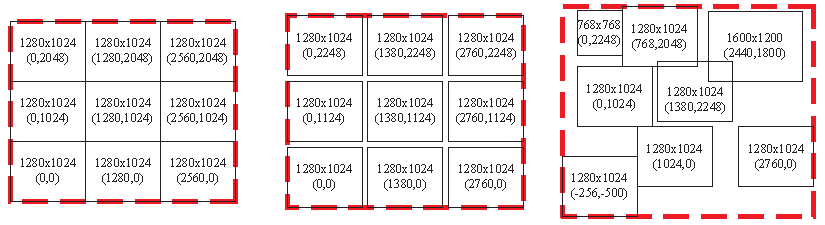
\includegraphics{images/ExampleTileConfig}
  \caption[Defining a tile display.]{Defining a tile display with viewports
    in a logical global display.  Three possible tile arrangements are
    shown.  The bounds of each tile is drawn with the viewport given
    inside.  The viewable area is shown with a dashed line.}
  \label{fig:BasicUsage:tile_layout}
\end{figure}

Figure~\ref{fig:BasicUsage:tile_layout} shows some possible tile
arrangements.  Mullions or overlaps of the tiles in the physical display
can be represented by the spacing or overlap of the viewports in the
logical display.  \IceT does not require the tile layout to have any
regularity.  Chaotic layouts like that shown in the right image of
Figure~\ref{fig:BasicUsage:tile_layout} are legal, although probably not
very useful.  It is allowed, and in fact encouraged, to have processes that
are not directly connected to the tiled display.  These
\index{non-display~process}\keyterm{non-display} processes still contribute
to the image compositing work and will reduce the overall time to render an
image.

The display is defined using the \CFunc{icetResetTiles} and
\CFunc{icetAddTile} functions.  Any previous tile definition is first
cleared out using \CFunc{icetResetTiles} and new tiles are added, one at a
time, using \CFunc{icetAddTile}.

\begin{Table}{3}
  \textC{void }\CFunc{icetResetTiles}\textC{(}&\textC{void}&\textC{)}
\end{Table}

\begin{Table}{3}
  \textC{int }\CFunc{icetAddTile}\textC{(}&\textC{IceTInt}&\CArg{x}\textC{,} \\
    &\textC{IceTInt}&\CArg{y}\textC{,} \\
    &\textC{IceTSizeType}&\CArg{width}\textC{,} \\
    &\textC{IceTSizeType}&\CArg{height}\textC{,} \\
    &\textC{int}&\CArg{display\_rank}\quad\textC{);}
\end{Table}

Each tile is specified using screen coordinates in the logical global
display: the position of the lower left corner and the width and height of
the tile.  Each tile also has a \index{display~process}\keyterm{display
  process} associated with it.  After an image is completely rendered and
composited, the screen section belonging to this tile will be placed in the
process at the given rank.

The following code demonstrates a common example for establishing the tile
layout: a grid of projectors.  The arrangement of projectors in this
example assume that the projectors are connected to processes in the order
of left to right and then top to bottom, which is common.  Note, however,
that \IceT defines its logical global display with $y$ values from the
bottom up like OpenGL does.

\begin{code}
  icetResetTiles();
  for (row = 0; row < num_tile_rows; row++) {
      for (column = 0; column < num_tile_columns; column++) {
          icetAddTile(column*TILE_WIDTH, (num_tile_rows-row-1)*TILE_HEIGHT,
                      TILE_WIDTH, TILE_HEIGHT,
                      row*num_tile_columns + column);
      }
  }
\end{code}

\index{mullion}\keyterm{Mullions} are added by simply spacing the tiles
apart from each other in the logical global display.  Because they are
defined in the logical global display, physical dimensions of the mullions
must first be converted to pixels using the dot pitch of the displays.  The
following code adds mullions between all of the tiles.

\begin{code}
  icetResetTiles();
  for (row = 0; row < num_tile_rows; row++) {
      for (column = 0; column < num_tile_columns; column++) {
          icetAddTile(column*(TILE_WIDTH + x_mullion),
                      (num_tile_rows-row-1)*(TILE_HEIGHT + y_mullion),
                      TILE_WIDTH, TILE_HEIGHT,
                      row*num_tile_columns + column);
      }
  }
\end{code}

An equally common use for \IceT is to render images in parallel to a single
display.  In this \index{single-tile~rendering}\keyterm{single-tile
  rendering} mode, we simply create a single tile whose image will be
placed in the GUI of some application.  This is done by either using the
OpenGL context of the GUI as part of the \IceT rendering process or by
grabbing the image of the single tile and copying into the GUI.  The
example code below sets up \IceT to create a single image that is
accessible on the root process.

\begin{code}
  icetResetTiles();
  icetAddTile(0, 0, SCREEN_WIDTH, SCREEN_HEIGHT, 0);
\end{code}

\IceT indexes the tiles in the order that they are defined with
\CFunc{icetAddTile}.  You can get the current definition of the tile
display from a number of state variables, which can be retrieved as always
with \CFunc{icetGet}.  \CEnum{ICET\_NUM\_TILES} stores the number of tiles
that are defined (the number of times \CFunc{icetAddTile} was called).
\CEnum{ICET\_TILE\_VIEWPORTS} stores an array with all of the dimensions of
each tile.  For each tile, \CEnum{ICET\_TILE\_VIEWPORTS} contains the four
\index{viewport}values $\langle x, y, width, height \rangle$, stored
consecutively, corresponding to the values passed to \CFunc{icetAddTile}.
\CEnum{ICET\_DISPLAY\_NODES} stores an array giving the rank of the
\index{display~process}display process displaying that tile.  Each process
can also query the \CEnum{ICET\_TILE\_DISPLAYED} variable to see which tile
is displayed locally.  \CEnum{ICET\_TILE\_DISPLAYED} is set to $-1$ on
every process that does not display a tile.

You can get information about the display geometry as a whole through
\CEnum{ICET\_GLOBAL\_VIEWPORT}.  This variable stores the four-tuple
$\langle x, y, width, height \rangle$.  $x$ and $y$ are placed at the
leftmost and lowest position of all the tiles, and $width$ and $height$ are
just big enough for the viewport to cover all tiles.

The \IceT image compositor remains decoupled from the rendering system.
Calling \CFunc{icetAddTile} will not create a display context or renderable
window for the tile.  That responsibility is left to the calling
application.  When using \IceT in \index{single-tile~rendering}single-tile
rendering mode, the rendering system should be set to produce images of
that single tile's size.  When driving a physical tiled display, each
display process must create a window that covers the entire display.  It is
also a good idea to disable the mouse cursor in these windows.

Note that the size of the tiles do not have to match each other.  Also, the
size of the images that your application generates do not have to match the
size of any of the tiles.  There is, however, a constraint that the
generated images on all processes must be at least as large as the largest
tile in each dimension.  To help you maintain that constraint, \IceT stores
the largest tile dimensions in the \CEnum{ICET\_TILE\_MAX\_WIDTH} and
\CEnum{ICET\_TILE\_MAX\_HEIGHT} state variables.

\IceT must know in advanced the size of images that your application will
render.  If you are using \IceT's \OpenGL layer, \IceT will automatically
know the size of the images you generate based off of the current \OpenGL
viewport (retrieved with the \CEnum{GL\_VIEWPORT} \OpenGL state variable).
Otherwise, you can specify the size of images the application generates
with \CFunc{icetPhysicalRenderSize}.  If you are not using the \OpenGL
layer and you have not called \CFunc{icetPhysicalRenderSize}, \IceT assumes
that you will generate images of width \CEnum{ICET\_TILE\_MAX\_WIDTH} and
height \CEnum{ICET\_TILE\_MAX\_HEIGHT}.  The actual expected rendered image
size is stored in the \CEnum{ICET\_PHYSICAL\_RENDER\_WIDTH} and
\CEnum{ICET\_PHYSICAL\_RENDER\_HEIGHT} state variables.

Although counterintuitive, it is often more efficient to create images that
are larger than any tile.  This situation may be necessary when using
\index{image!inflation}image inflation (see
Chapter~\ref{sec:Customizing_Compositing:Image_Inflation}).  Even when not
using image inflation, larger rendered images can save a significant amount
of rendering time.  \IceT can use the larger images to potentially render
in one shot an object that is larger than any of the tiles.

\index{display~definition|)}
\index{tile~definition|)}


\section{Strategies}
\label{sec:Basic_Usage:Strategies}

\index{strategy|(}

\IceT contains several algorithms for performing image compositing.  The
overall algorithm used to render and composite an image is called a
strategy, named after the ``Gang of Four'' strategy pattern.\footnote{Erich
  Gamma, Richard Helm, Ralph Johnson, and John Vlissides.  \emph{Design
    Patterns}.  Addison-Wesley, 1994.  ISBN 0-201-63361-2.}  The strategy
is set using the \CFunc{icetStrategy} function.

\begin{Table}{3}
  \textC{void }\CFunc{icetStrategy}\textC{(}&\textC{IceTEnum}&\CArg{strategy}\quad\textC{);}
\end{Table}

\IceT defines the following strategies that can be passed to
\CFunc{icetStrategy}.  These strategies are discussed in more detail in
Chapter~\ref{chap:Strategies}.

% -*- latex -*-

  \begin{Description}
  \item[\CEnum{ICET\_STRATEGY\_SEQUENTIAL}]
    Basically applies a ``traditional'' single tile composition (such as
    binary swap) to each tile in the order they were defined.  Because each
    process must take part in the composition of each tile regardless of
    whether they draw into it, this strategy is usually inefficient when
    compositing for more than one tile, but is recommended for the single
    tile case because it bypasses some of the communication necessary for
    the other multi-tile strategies.
    \index{strategy!sequential}
  \item[\CEnum{ICET\_STRATEGY\_DIRECT}] As each process renders an image
    for a tile, that image is sent directly to the process that will
    display that tile.  This usually results in a few processes receiving
    and processing the majority of the data, and is therefore usually an
    inefficient strategy.
    \index{strategy!direct}
  \item[\CEnum{ICET\_STRATEGY\_SPLIT}] Like \CEnum{ICET\_STRATEGY\_DIRECT},
    except that the tiles are split up, and each process is assigned a
    piece of a tile in such a way that each process receives and handles
    about the same amount of data.  This strategy is often very efficient,
    but due to the large amount of messages passed, it has not proven to be
    very scalable or robust.
    \index{strategy!split}
  \item[\CEnum{ICET\_STRATEGY\_REDUCE}] A two phase algorithm.  In the
    first phase, tile images are redistributed such that each process has
    one image for one tile.  In the second phase, a ``traditional'' single
    tile composition is performed for each tile.  Since each process
    contains an image for only one tile, all these compositions may happen
    simultaneously.  This is a well rounded strategy that seems to perform
    well in a wide variety of multi-tile applications.  (However, in the
    special case where only one tile is defined, the sequential strategy is
    probably better.)
    \index{strategy!reduce}
  \item[\CEnum{ICET\_STRATEGY\_VTREE}] An extension to the binary tree
    algorithm for image composition.  Sets up a ``virtual'' composition
    tree for each tile image.  Processes that belong to multiple trees
    (because they render to more than one tile) are allowed to float
    between trees.  This strategy is not quite as well load balanced as
    \CEnum{ICET\_STRATEGY\_REDUCE} or \CEnum{ICET\_STRATEGY\_SPLIT}, but
    has very well behaved network communication.
    \index{strategy!virtual~trees}
  \end{Description}


You can get a human-readable name using the \CFunc{icetGetStrategyName}
function.

\begin{Table}{3}
  \textC{const char *}\CFunc{icetGetStrategyName}\textC{(}&\textC{void}&\textC{);}
\end{Table}

The algorithms in \IceT's strategies are specially designed to composite
data defined on multiple tiles.  Some of these algorithms, namely
\CEnum{ICET\_STRATEGY\_REDUCE} and \CEnum{ICET\_STRATEGY\_SEQUENTIAL},
operate at least in part by compositing single images together.  \IceT also
comes with multiple separate strategies for performing this single image
compositing, and this can be selected with the
\CFunc{icetSingleImageStrategy} function.

\begin{Table}{3}
  \textC{void }\CFunc{icetSingleImageStrategy}\textC{(}&\textC{IceTEnum}&\CArg{strategy}\quad\textC{);}
\end{Table}

\IceT defines the following single image strategies that can be passed to
\CFunc{icetSingleImageStrategy}.  These strategies are discussed in more
detail in Chapter~\ref{chap:Strategies}.

% -*- latex -*-

\begin{Description}
\item[\CEnum{ICET\_SINGLE\_IMAGE\_STRATEGY\_AUTOMATIC}] Automatically
  chooses which single image strategy to use based on the number of
  processes participating in the composition.
  \index{single~image~strategy!automatic}
\item[\CEnum{ICET\_SINGLE\_IMAGE\_STRATEGY\_BSWAP}] The classic binary swap
  compositing algorithm.  At each phase of the algorithm, each process
  partners with another, sends half of its image to its partner, and
  receives the opposite half from its partner.  The processes are then
  partitioned into two groups that each have the same image part, and the
  algorithm recurses.
  \index{single~image~strategy!binary~swap}
\item[\CEnum{ICET\_SINGLE\_IMAGE\_STRATEGY\_TREE}] At each phase, each
  process partners with another, and one of the processes sends its entire
  image to the other.  The algorithm recurses with the group of processes
  that received images until only one process has an image.
  \index{single~image~strategy!tree}
\end{Description}


By default \IceT sets the single image strategy to
\CEnum{ICET\_SINGLE\_IMAGE\_STRATEGY\_AUTOMATIC} when a context is created.
This is the single image strategy that will be used if no other is
selected.

You can get a human-readable name using the
\CFunc{icetGetSingleImageStrategyName} function.

\begin{Table}{3}
  \textC{const char *}\CFunc{icetGetSingleImageStrategyName}\textC{(}&\textC{void}&\textC{);}
\end{Table}

\index{strategy|)}


\section{Drawing Callback}
\label{sec:Basic_Usage::Drawing_Callback}

\index{drawing~callback|(}

Most compositing engines will simply take a group of images and combine them
together.  This approach, however, is unreasonable when compositing the
high resolution images on a large tiled display.  It is problematic for an
application to create images larger than any color buffer the rendering
hardware can create, and holding many of these large images can lead to a
large memory profile.

Instead, the \IceT algorithms deal with pieces of the overall image.  The
image pieces are created on demand.  As such, \IceT may require the same
geometry to be rendered multiple times in a single frame.  \IceT provides
the application with the most flexible way to define the rendering process:
with a \keyterm{drawing callback}.

A drawing callback is simply a function that your application provides
\IceT.  When \IceT needs an image, it will provide the drawing callback
with the projection matrices for the section of the display being
rendered.  The drawing callback then returns the image rendered to those
projection matrices.

\IceT may call the drawing callback several times to create a single tiled
image or not at all if the current bounds lie outside the current view
frustum.  This can have a subtle but important impact on the behavior of
the drawing callback.  For example, counting frames by incrementing a frame
counter in the drawing callback is obviously wrong (although you could
count how many times a render occurs).  The drawing callback should also
leave the rendering system in a state such that it will be correct for a
subsequent run of the drawing callback.  Any state that is assumed to be
true on entrance to the drawing callback should also be true on return.

\subsection{Generic Drawing Callback}
\label{sec:Basic_Usage:Drawing_Callback:Generic}

There are two versions of drawing callbacks.  The first version is a
generic callback set with \CFunc{icetDrawCallback}.  This callback is used
in conjunction with the \CFunc{icetDrawFrame} function (described in the
next section).

\begin{Table}{3}
  \multicolumn{3}{l}{
    \textC{typedef void (*}\CType{IceTDrawCallbackType}\textC{)(}
  } \\
  \qquad\qquad\qquad\qquad\qquad\qquad\qquad\qquad
  &\textC{const IceTDouble *}&\CArg{projection\_matrix}\textC{,} \\
  &\textC{const IceTDouble *}&\CArg{modelview\_matrix}\textC{,} \\
  &\textC{const IceTFloat *}&\CArg{background\_color}\textC{,} \\
  &\textC{const IceTInt *}&\CArg{readback\_viewport}\textC{,} \\
  &\CType{IceTImage}&\CArg{result}\quad\textC{)}
\end{Table}

\begin{Table}{3}
  \textC{void }\CFunc{icetDrawCallback}\textC{(}&\CType{IceTDrawCallbackType}&\CArg{callback}\quad\textC{);}
\end{Table}

\CArg{callback} takes two projection matrices: \CArg{projection\_matrix}
and \CArg{modelview\_matrix}.  Each of these arguments is a 16-value array
that represents a $4 \times 4$ transformation of homogeneous coordinates.
The arrays store the matrices in \index{column-major~order}column-major
order.  Thus, if the values in \CArg{projection\_matrix} are $(p[0],
p[1],... p[15])$ and the values in \CArg{modelview\_matrix} are $(m[0],
m[1],... m[15])$, then a vertex in object space is transformed into
normalized screen coordinates by the sequence of operations

\begin{displaymath}
  \left[
    \begin{array}{cccc}
      p[0] & p[4] & p[8] & p[12] \\
      p[1] & p[5] & p[9] & p[13] \\
      p[2] & p[6] & p[10] & p[14] \\
      p[3] & p[7] & p[11] & p[15]
    \end{array}
  \right]
  \left[
    \begin{array}{cccc}
      m[0] & m[4] & m[8] & m[12] \\
      m[1] & m[5] & m[9] & m[13] \\
      m[2] & m[6] & m[10] & m[14] \\
      m[3] & m[7] & m[11] & m[15]
    \end{array}
  \right]
  \left[
    \begin{array}{c}
      v[0] \\ v[1] \\ v[2] \\ v[3]
    \end{array}
  \right]
\end{displaymath}

More explicitly, if you have a point $(x, y, z, 1)$ in object space stored
in a variable \textC{object\_coord}, you could transform that to world
space in the callback with code like this.

\begin{code}
for (row = 0; row < 4; row++) {
    world_coord[row] = 0.0;
    for (i = 0; i < 4; i++) {
        world_coord[row] += modelview_matrix[row + 4*i] * object_coord[i];
    }
}
\end{code}

Likewise, to transform the \textC{world\_coord} to normalized screen
coordinates, you could apply the following code.

\begin{code}
for (row = 0; row < 4; row++) {
    screen_coord[row] = 0.0;
    for (i = 0; i < 4; i++) {
        screen_coord[row] += projection_matrix[row + 4*i] * world_coord[i];
    }
}
\end{code}

If your rendering system has no need to find the world coordinates of
points, you can combine the two matrices by multiplying them together like
this.

\begin{code}
for (row = 0; row < 4; row++) {
    for (column = 0; column < 4; column++) {
        full_matrix[row + 4*column] = 0.0;
        for (i = 0; i < 4; i++) {
            full_matrix[row + 4*column] +=
                projection_matrix[row + 4*i] * modelview_matrix[k + 4*column];
        }
    }
}
\end{code}

Normalized screen coordinates are such that everything projected onto the
image has coordinates in the range $[-1,1]$ (after dividing by the ``w''
homogeneous coordinate).  The x and y coordinates have to be shifted to get
the corresponding pixel location.  The normalized screen coordinates are
projected to span the physical render size (see
\CFunc{icetPhysicalRenderSize}), which may differ from the size of any
particular tile.  Also, if you are outputting depth values, \IceT expects
values in the range $[0,1]$, so you will have to shift those as well.  Here
is a pedantic code segment to do this final transformation.

\begin{code}
icetGetIntegerv(ICET_PHYSICAL_RENDER_WIDTH, &image_width);
icetGetIntegerv(ICET_PHYSICAL_RENDER_HEIGHT, &image_height);
/* Alternatively, you could get the width and height from the image passed */
/* to the callback like this.                                              */
/* image_width = icetImageGetWidth(result);                                */
/* image_height = icetImageGetHeight(result);                              */
pixel_x = (int)(image_width*0.5*(screen_coord[0]/screen_coord[3] + 1.0));
pixel_y = (int)(image_height*0.5*(screen_coord[1]/screen_coord[3] + 1.0));
depth = 0.5*(screen_coord[2]/screen_coord[3] + 1.0);
\end{code}

The drawing callback should initialize its backdrop to the
\CArg{background\_color}, which may be different than the background color
passed to \CFunc{icetDrawFrame}.

The resulting image should be rendered (or copied) into the
\CType{IceTImage}, \CArg{result}, passed to the callback.  The image will
be sized by the physical render width and height and its format will
conform to that set by \CFunc{icetSetColorFormat} and
\CFunc{icetSetDepthFormat}.  You can get the buffers of the image with the
\icetImageGetColor and \icetImageGetDepth functions.  Data written to these
buffers will become part of the image.  \IceT's image functions are
described in more detail in the following section starting on
page~\pageref{sec:Basic_Usage:Image_Objects}.

\IceT will always send the drawing callback an image sized by the physical
render viewport specified by \CFunc{icetPhysicalRenderSize} for
convenience.  However, \IceT often needs only a subset of these pixels.
\IceT tells the drawing callback the pixels it actually uses with the
\CArg{readback\_viewport} parameter.  \CArg{readback\_viewport} contains 4
integers specifying a region of pixels that \IceT will use.  The first two
value specify the lower-left corner of the region and the next two specify
the width and height of the region.

For example, if the \CArg{readback\_viewport} is set to $(10, 15, 100,
75)$, then \IceT will use only the pixels in the square between x values 10
and 109 and y values between 15 and 89 (both inclusive).  All other pixels
in the image will be ignored.  It is not an error to provide values for the
other pixels, but it is a waste of computation.

\subsection{OpenGL Drawing Callback}
\label{sec:Basic_Usage:Drawing_Callback:OpenGL}

If you are rendering with \OpenGL, then you can remove many of the
complexities of defining a callback by using \CFunc{icetGLDrawCallback} in
conjunction with \CFunc{icetGLDrawFrame}.

\textC{typedef void (*} \CType{IceTGLDrawCallbackType}\textC{)( void );}

\begin{Table}{3}
  \textC{void }\CFunc{icetGLDrawCallback}\textC{(}&\CType{IceTGLDrawCallbackType}&\CArg{callback}\quad\textC{);}
\end{Table}

The \OpenGL version of the drawing callback takes no arguments.  It simply
issues the appropriate \OpenGL calls to render the geometry.  \IceT
internally takes care of setting the appropriate transformations and clear
color, and then reads back your data from the buffer specified by
\CFunc{icetGLSetReadBuffer} after the drawing callback returns.

The \OpenGL drawing callback should \emph{not} modify the
\CEnum{GL\_PROJECTION\_MATRIX} as this would cause \IceT to place image
data in the wrong location in the tiled display and improperly cull
geometry.  It is acceptable to add transformations to
\CEnum{GL\_MODELVIEW\_MATRIX}, but the bounding vertices given with
\CFunc{icetBoundingVertices} or \CFunc{icetBoundingBox} (see the following
section) are assumed to already be transformed by any such changes to the
modelview matrix.  Also, \CEnum{GL\_MODELVIEW\_MATRIX} must be restored
before the draw function returns.  Therefore, any changes to
\CEnum{GL\_MODELVIEW\_MATRIX} are to be done with care and should be
surrounded by a pair of glPushMatrix and glPopMatrix functions.

It is also important that the \OpenGL drawing callback \emph{not} attempt
the change the clear color.  In some compositing modes, \IceT needs to
read, modify, and change the background color.  These operations will be
lost if the drawing callback changes the background color, and severe color
blending artifacts may result.

\subsection{Specifying Geometry Bounds}
\label{sec:Basic_Usage:Drawing_Callback:Bounds}

\IceT can nominally call the drawing callback for every tile in the
display.  However, in almost any real application each process has data
that demonstrates some spatial locality that causes it to be projected on a
relatively small section of the display.  To give \IceT the information it
needs to prevent unnecessary renders, the application needs to provide the
bounds of the local geometry.  This is done using either the
\CFunc{icetBoundingVertices} or the \CFunc{icetBoundingBox} function.

\begin{Table}{3}
  \textC{void }\CFunc{icetBoundingVertices}\textC{(}&\textC{IceTInt}&\CArg{size}\textC{,} \\
    &\textC{IceTEnum}&\CArg{type}\textC{,} \\
    &\textC{IceTSizeType}&\CArg{stride}\textC{,} \\
    &\textC{IceTSizeType}&\CArg{count}\textC{,} \\
    &\textC{const IceTVoid *}&\CArg{pointer}\quad\textC{);}
\end{Table}

\begin{Table}{3}
  \textC{void }\icetBoundingBoxd\textC{(}&\textC{IceTDouble}&\CArg{x\_min}\textC{,} \\
    &\textC{IceTDouble}&\CArg{x\_max}\textC{,} \\
    &\textC{IceTDouble}&\CArg{y\_min}\textC{,} \\
    &\textC{IceTDouble}&\CArg{y\_max}\textC{,} \\
    &\textC{IceTDouble}&\CArg{z\_min}\textC{,} \\
    &\textC{IceTDouble}&\CArg{z\_max}\quad\textC{);}
\end{Table}

\begin{Table}{3}
  \textC{void }\icetBoundingBoxf\textC{(}&\textC{IceTFloat}&\CArg{x\_min}\textC{,} \\
    &\textC{IceTFloat}&\CArg{x\_max}\textC{,} \\
    &\textC{IceTFloat}&\CArg{y\_min}\textC{,} \\
    &\textC{IceTFloat}&\CArg{y\_max}\textC{,} \\
    &\textC{IceTFloat}&\CArg{z\_min}\textC{,} \\
    &\textC{IceTFloat}&\CArg{z\_max}\quad\textC{);}
\end{Table}

With the \CFunc{icetBoundingVertices} function, you specify a set of
vertices whose convex hull completely contains the geometry.  The
\CFunc{icetBoundingBox} function is a convenience function that defines the
container as an axis aligned bounding box.

\index{drawing~callback|)}


\section{Rendering}
\label{sec:Basic_Usage:Rendering}

Once you have set up the \IceT state as described in the previous sections
of this chapter, you are ready to perform parallel rendering.  Rendering is
initiated in \IceT by calling one of the draw frame functions.

\subsection{Generic Rendering}
\label{sec:Basic_Usage:Rendering:Generic}

There are two frame drawing functions.  The first version is independent of
the rendering system and is used in conjunction with the callback set with
\CFunc{icetDrawCallback}.  It is performed by calling
\CFunc{icetDrawFrame}.

\begin{Table}{3}
  \CType{IceTImage}\textC{ }\CFunc{icetDrawFrame}\textC{(}
  &\textC{const IceTDouble *}&\CArg{projection\_matrix}\textC{,} \\
  &\textC{const IceTDouble *}&\CArg{modelview\_matrix}\textC{,} \\
  &\textC{const IceTFloat *}&\CArg{background\_color}\quad\textC{);}
\end{Table}

Conceptually, calling \CFunc{icetDrawFrame} is similar to calling the
\index{drawing~callback}drawing callback directly.  The arguments
\CArg{projection\_matrix}, \CArg{modelview\_matrix}, and
\CArg{background\_color} are the same as you would potentially pass the
callback (although \IceT is free to change them).

The \CArg{projection\_matrix} and \CArg{modelview\_matrix} are 16-value
arrays that represent $4 \times 4$ transformations of homogeneous coordinates.
The arrays store the matrices in \index{column-major~order}column-major
order.  Thus, if the values in \CArg{projection\_matrix} are $(p[0],
p[1],... p[15])$ and the values in \CArg{modelview\_matrix} are $(m[0],
m[1],... m[15])$, then a vertex in object space is transformed into
normalized screen coordinates by the sequence of operations

For example, if your modelview matrix used a simple translation to move the
geometry in front of the camera, you would use a matrix like this.

\begin{displaymath}
  \left[
    \begin{array}{cccc}
      1 & 0 & 0 & x \\
      0 & 1 & 0 & y \\
      0 & 0 & 1 & z \\
      0 & 0 & 0 & 1
    \end{array}
  \right]
\end{displaymath}

The code to set the modelview matrix could look like this.

\begin{code}
modelview_matrix[ 0] = 1.0;
modelview_matrix[ 1] = 0.0;
modelview_matrix[ 2] = 0.0;
modelview_matrix[ 3] = 0.0;

modelview_matrix[ 4] = 0.0;
modelview_matrix[ 5] = 1.0;
modelview_matrix[ 6] = 0.0;
modelview_matrix[ 7] = 0.0;

modelview_matrix[ 8] = 0.0;
modelview_matrix[ 9] = 0.0;
modelview_matrix[10] = 1.0;
modelview_matrix[11] = 0.0;

modelview_matrix[12] = x;
modelview_matrix[13] = y;
modelview_matrix[14] = z;
modelview_matrix[15] = 1.0;
\end{code}

As another example, consider setting the projection matrix for the
perspective of a camera sitting at the origin facing down the $-z$ axis.
You could use a transformation matrix like this.

\begin{displaymath}
  \begin{array}{c}
    \left[
      \begin{array}{cccc}
        \frac{f \cdot height}{width} & 0 & 0 & 0 \\
        0 & f & 0 & 0 \\
        0 & 0 & -1 & -2near \\
        0 & 0 & -1 & 0
      \end{array}
    \right] \\
    f = \mathrm{cotangent}\left(\frac{fovy}{2}\right)
  \end{array}
\end{displaymath}

The code to set the projection matrix could look like this.

\begin{code}
/* width, height: image dimensions */
/* fovy: field of view in the y direction */
/* zNear: distance from camera (at origin) to near clipping plane (at -zNear). */

f = 1.0/tan(0.5*fovy);

projection_matrix[ 0] = (f*height)/width;
projection_matrix[ 1] = 0.0;
projection_matrix[ 2] = 0.0;
projection_matrix[ 3] = 0.0;

projection_matrix[ 4] = 0.0;
projection_matrix[ 5] = f;
projection_matrix[ 6] = 0.0;
projection_matrix[ 7] = 0.0;

projection_matrix[ 8] = 0.0;
projection_matrix[ 9] = 0.0;
projection_matrix[10] = -1.0;
projection_matrix[11] = -1.0;

projection_matrix[12] = 0.0;
projection_matrix[13] = 0.0;
projection_matrix[14] = -2*zNear;
projection_matrix[15] = 0.0;
\end{code}

The \CArg{background\_color} is the color in which the background should be
initialized.  It is the color of ``empty'' pixels and also the color to be
blended with any transparent geometry.

\CFunc{icetDrawFrame} returns an \CType{IceTImage} containing the composited
image displayed on this process.  If the process is not displaying a tile,
then the contents of the image is undefined.

\subsection{OpenGL Rendering}
\label{sec:Basic_Usage:Rendering:OpenGL}

If you are rendering with \OpenGL, then you can remove many of the
complexities of defining projection matrices and displaying images by using
the \CFunc{icetGLDrawFrame} function in conjunction with the drawing
callback set with \CFunc{icetGLDrawCallback}.

\begin{Table}{3}
  \textC{void}\quad\CFunc{icetGLDrawFrame}\textC{( void );}
\end{Table}

\CFunc{icetGLDrawFrame} is called in basically the same way as the \OpenGL
\index{drawing~callback}drawing callback would be called directly.  First,
establish the \OpenGL state.  Setting up the \CEnum{GL\_PROJECTION\_MATRIX}
before calling \CFunc{icetGLDrawFrame} is essential.  It is also advisable
to set up whatever transformations in the \CEnum{GL\_MODELVIEW\_MATRIX}
that you can before calling \CFunc{icetGLDrawFrame}.  \IceT will use and
modify these two matrices to render regions of the tiled display.  The
drawing callback should behave as if neither of the matrices were modified.

By the time \CFunc{icetGLDrawFrame} completes, an image will have been
completely rendered and composited.  If \CEnum{ICET\_GL\_DISPLAY} is
enabled, then the fully composited image is written back to the \OpenGL
frame buffer for display.  It is the application's responsibility to
synchronize the processes and swap front and back buffers.  The image
remaining in the frame buffer is undefined if \CEnum{ICET\_GL\_DISPLAY} is
disabled or the process is not displaying a tile.

If the \OpenGL background color is set to something other than black,
\CEnum{ICET\_GL\_DISPLAY\_COLORED\_BACKGROUND} should also be enabled.
Displaying with \CEnum{ICET\_GL\_DISPLAY\_COLORED\_BACKGROUND} disabled may
be slightly faster (depending on graphics hardware) but can result in black
rectangles in the background.

If \CEnum{ICET\_GL\_DISPLAY\_INFLATE} is enabled and the size of the
renderable window (determined by the current \OpenGL viewport) is greater
than that of the tile being displayed, then the image will first be
``inflated'' to the size of the actual display.  If
\CEnum{ICET\_GL\_DISPLAY\_INFLATE} is disabled, the image is drawn at its
original resolution at the lower left corner of the display.  More details
on image inflation are given in
Chapter~\ref{sec:Customizing_Compositing:Image_Inflation}.

Regardless of whether it writes the fully composited image back to the
display, \CFunc{icetGLDrawFrame} returns an \CType{IceTImage} containing
the composited image displayed on this process.  If the process is not
displaying a tile, then the contents of the image is undefined.


\section{Image Objects}
\label{sec:Basic_Usage:Image_Objects}

\IceT uses a data type called \CType{IceTImage} to store and pass around
image data.  To get image data from a generic drawing callback (described
previously starting on
page~\pageref{sec:Basic_Usage:Drawing_Callback:Generic}), \IceT passes the
callback an \CType{IceTImage} sized to hold an image of the appropriate
dimensions.  Likewise, the frame drawing functions (described previously
starting on page~\pageref{sec:Basic_Usage:Rendering}) return an
\CType{IceTImage}.  An \CType{IceTImage} is intended to be an opaque object
that is accessed by a suite of functions provided by \IceT.

\index{null image|see{image, null}}

\IceT defines a special \index{image!null}\keyterm{null image} that can be
used as a place holder when no image data is available.  You can create and
check for null images with the \CFunc{icetImageNull} and
\CFunc{icetImageIsNull} functions, respectively.

\begin{Table}{3}
  \CType{IceTImage}\textC{ }\CFunc{icetImageNull}\textC{(}&\textC{void}&\textC{);}
\end{Table}
\begin{Table}{3}
  \textC{IceTBoolean}\textC{ }\CFunc{icetImageIsNull}\textC{(}&\CType{IceTImage}&\CArg{image}\quad\textC{);}
\end{Table}

It is good defensive programming to initialize \CType{IceTImage} objects to
null on creation.  That way, all of \IceT's images functions will always
behave appropriately on the image, whereas the behavior is unpredictable if
the \CType{IceTImage} is uninitialized.

\begin{code}
  IceTImage image = icetImageNull();
\end{code}

The functions \CFunc{icetImageGetWidth}, \CFunc{icetImageGetHeight}, and
\CFunc{icetImageGetNumPixels} return the dimensions of an image.

\begin{Table}{5}
  \textC{IceTSizeType}&\icetImageGetWidth&\textC{(}\quad\textC{const }\CType{IceTImage}&\CArg{image}&\textC{);} \\
  \textC{IceTSizeType}&\icetImageGetHeight&\textC{(}\quad\textC{const }\CType{IceTImage}&\CArg{image}&\textC{);} \\
  \textC{IceTSizeType}&\icetImageGetNumPixels&\textC{(}\quad\textC{const }\CType{IceTImage}&\CArg{image}&\textC{);}
\end{Table}

An \CType{IceTImage} can hold color data, depth data, or both.
Furthermore, colors and depths can be stored in different formats.  The
internal formats for colors and depths for an \CType{IceTImage} can be
retrieved with the \CFunc{icetImageGetColorFormat} and
\CFunc{icetImageGetDepthFormat} functions, respectively.

\begin{Table}{5}
  \textC{IceTEnum}&\icetImageGetColorFormat\textC{(}&\textC{const }\CType{IceTImage}&\CArg{image}&\textC{);} \\
  \textC{IceTEnum}&\icetImageGetDepthFormat\textC{(}&\textC{const }\CType{IceTImage}&\CArg{image}&\textC{);}
\end{Table}

The format specifies the basic data type, the packing, and whether the
color or depth data is available at all.  Here is a list of possible color
formats.

% -*- latex -*-

  \begin{Description}[ICET\_IMAGE\_COLOR\_RGBA\_UBYTE]
  \item[\CEnum{ICET\_IMAGE\_COLOR\_RGBA\_UBYTE}] Each entry is an RGBA
    color tuple.  Each component is valued in the range from $0$ to $255$
    and is stored as an 8-bit integer.  The buffer will always be allocated
    on memory boundaries such that each color value can be treated as a
    single 32-bit integer.
  \item[\CEnum{ICET\_IMAGE\_COLOR\_RGBA\_FLOAT}] Each entry is an RGBA
    color tuple.  Each component is in the range from $0.0$ to $1.0$ and is
    stored as a 32-bit float.
  \item[\CEnum{ICET\_IMAGE\_COLOR\_RGB\_FLOAT}] Each entry is an RGB color
    triple. Each component is in the range from $0.0$ to $1.0$ and is
    stored as a 32-bit float. Note that there is no alpha channel, so the
    color blending composite mode will not work with this color format.
  \item[\CEnum{ICET\_IMAGE\_COLOR\_NONE}] No color values are stored in the
    image.
  \end{Description}



Here is a list of possible depth formats.

% -*- latex -*-

  \begin{Description}[ICET\_IMAGE\_COLOR\_RGBA\_UBYTE]
  \item[\CEnum{ICET\_IMAGE\_DEPTH\_FLOAT}] Each entry is in the range from
    $0.0$ (near plane) to $1.0$ (far plane) and is stored as a 32-bit
    float.
  \item[\CEnum{ICET\_IMAGE\_DEPTH\_NONE}] No depth values are stored in the
    image.
  \end{Description}


An \CType{IceTImage} stores the color and depth data in separate buffers.
You can use the \icetImageGetColor and \icetImageGetDepth functions to
retrieve pointers to this data.  A drawing callback must use these
functions to get buffers to write data into.

\begin{Table}{4}
  \textC{IceTUByte *}&\icetImageGetColorub&\textC{(}\quad\CType{IceTImage}&\CArg{image}\quad\textC{)}; \\
  \textC{IceTUInt *}&\icetImageGetColorui&\textC{(}\quad\CType{IceTImage}&\CArg{image}\quad\textC{)}; \\
  \textC{IceTFloat *}&\icetImageGetColorf&\textC{(}\quad\CType{IceTImage}&\CArg{image}\quad\textC{)}; \\
  \\
  \textC{IceTFloat *}&\icetImageGetDepthf&\textC{(}\quad\CType{IceTImage}&\CArg{image}\quad\textC{)};
\end{Table}

The various forms of \icetImageGetColor and \icetImageGetDepth return typed
arrays for the buffer of data.  The type of the data must conform to the
internal format of the data; the functions will raise an error otherwise.

If you want to use image data of a specific format, you can use one of the
\icetImageCopyColor or \icetImageCopyDepth functions.  With these
functions, you give an allocated array and a specific color format, and the
data for that array will be copied into your buffer in the desired format.

\begin{Table}{4}
  \textC{void}&\icetImageCopyColorub\textC{(}&\textC{const }\CType{IceTImage}&\CArg{image}\textC{,} \\
  &&\textC{IceTUByte *}&\CArg{color\_buffer}, \\
  &&\textC{IceTEnum}&\CArg{color\_format}\quad\textC{);} 
\end{Table}

\begin{Table}{4}
  \textC{void}&\icetImageCopyColorf\textC{(}&\textC{const }\CType{IceTImage}&\CArg{image}\textC{,} \\
  &&\textC{IceTFloat *}&\CArg{color\_buffer}, \\
  &&\textC{IceTEnum}&\CArg{color\_format}\quad\textC{);}
\end{Table}

\begin{Table}{4}
  \textC{void}&\icetImageCopyDepthf\textC{(}&\textC{const }\CType{IceTImage}&\CArg{image}\textC{,} \\
  &&\textC{IceTFloat *}&\CArg{depth\_buffer}, \\
  &&\textC{IceTEnum}&\CArg{depth\_format}\quad\textC{);}
\end{Table}



% -*- latex -*-

\chapter{Customizing Compositing}
\label{chap:Customizing_Compositing}

If you have been reading this document from the beginning, then you already
know enough to use \IceT for many typical rendering applications.  Chapters
\ref{chap:Tutorial} and \ref{chap:Basic_Usage} describe how to build and
link \IceT, establish an \IceT context in your application, and to leverage
\IceT to make your rendering parallel.  This chapter describes the many
features \IceT provides to let you customize the image compositing to your
application.

\section{Compositing Operation}
\label{sec:Customizing_Compositing:Compositing_Operation}
\index{compositing|(}
\index{compositing~operation|(}

\IceT is classified as a \index{sort-last}\keyterm{sort-last} type of
parallel rendering library, as discussed in
Chapter~\ref{sec:Introduction:Parallel_Rendering_Primer}.  Basically, this
means that each process renders images independently, and then these
images, each comprising a different partition of the geometry, are combined
together in a process called \keyterm{compositing}.

To combine two images together, a \keyterm{compositing operation} is
applied to every corresponding pair of pixels.  Three or more images are
combined by applying the compositing operation multiple times to eventually
reduce everything to one image.  (The compositing operations supported by
\IceT are associative, so the order is flexible.  \IceT takes advantage of
this fact to efficiently perform the compositing in parallel.)

\IceT supports two compositing operations, set with
\CFunc{icetCompositeMode}.

\begin{Table}{3}
  \textC{void }\CFunc{icetCompositeMode}\textC{(}&\textC{IceTEnum}&\CArg{mode}\quad\textC{);}
\end{Table}

The first type of compositing operation,
\CEnum{ICET\_COMPOSITE\_MODE\_Z\_BUFFER}, is a depth comparison and the
other, \CEnum{ICET\_COMPOSITE\_MODE\_BLEND}, is an alpha blend.  The depth
comparison is a bit faster and is easier to use, but only works for opaque
surfaces.  If you are performing \index{volume~rendering}\keyterm{volume
  rendering}, the translucent rendering of 3-dimensional volumes, or any
other rendering that involves transparent data, then you will have to use
the alpha blend compositing operation.

Each compositing operation relies on certain buffers to exist (or not
exist) in images.  For example, z-buffer compositing can use a color buffer
and requires a depth buffer whereas blended compositing requires a color
buffer and cannot work with a depth buffer.  The buffers created in images
by \IceT, and their formats, is controlled by the
\CFunc{icetSetColorFormat} and \CFunc{icetSetDepthFormat} functions.  It is
important to ensure that the setting for \CFunc{icetCompositeMode} is
compatible with the settings for \CFunc{icetSetColorFormat} and
\CFunc{icetSetDepthFormat}.

\begin{Table}{3}
  \textC{void }\icetSetColorFormat\textC{(}&\textC{IceTEnum}&\CArg{color\_format}\quad\textC{);} \\
  \textC{void }\icetSetDepthFormat\textC{(}&\textC{IceTEnum}&\CArg{depth\_format}\quad\textC{);}
\end{Table}

The following \CArg{color\_format}s are valid for use in
\CFunc{icetSetColorFormat}.

% -*- latex -*-

  \begin{Description}[ICET\_IMAGE\_COLOR\_RGBA\_UBYTE]
  \item[\CEnum{ICET\_IMAGE\_COLOR\_RGBA\_UBYTE}] Each entry is an RGBA
    color tuple.  Each component is valued in the range from $0$ to $255$
    and is stored as an 8-bit integer.  The buffer will always be allocated
    on memory boundaries such that each color value can be treated as a
    single 32-bit integer.
  \item[\CEnum{ICET\_IMAGE\_COLOR\_RGBA\_FLOAT}] Each entry is an RGBA
    color tuple.  Each component is in the range from $0.0$ to $1.0$ and is
    stored as a 32-bit float.
  \item[\CEnum{ICET\_IMAGE\_COLOR\_RGB\_FLOAT}] Each entry is an RGB color
    triple. Each component is in the range from $0.0$ to $1.0$ and is
    stored as a 32-bit float. Note that there is no alpha channel, so the
    color blending composite mode will not work with this color format.
  \item[\CEnum{ICET\_IMAGE\_COLOR\_NONE}] No color values are stored in the
    image.
  \end{Description}



The following \CArg{depth\_format}s are valid for use in
\CFunc{icetSetDepthFormat}.

% -*- latex -*-

  \begin{Description}[ICET\_IMAGE\_COLOR\_RGBA\_UBYTE]
  \item[\CEnum{ICET\_IMAGE\_DEPTH\_FLOAT}] Each entry is in the range from
    $0.0$ (near plane) to $1.0$ (far plane) and is stored as a 32-bit
    float.
  \item[\CEnum{ICET\_IMAGE\_DEPTH\_NONE}] No depth values are stored in the
    image.
  \end{Description}


\subsection{Z-Buffer Compositing}
\label{sec:Customizing_Compositing:User_Defined_Communicators}
\index{z-buffer}
\index{z-buffer|seealso{compositing, z-buffer}}
\index{depth~buffer|see{compositing, z-buffer}}
\index{compositing!z-buffer|(}

\keyterm{Z-buffer compositing} takes advantage of the same hidden surface
removal already taking place in the OpenGL pipeline.  \IceT pulls the
\index{z-buffer}z-buffer (also often known as the \keyterm{depth buffer})
from the OpenGL image buffers.  The compositing operation then just
compares the depth values of two pixels and chooses the one that is closer.

Z-buffer compositing is used when the composite mode (set with
\CFunc{icetCompositeMode}) is \CEnum{ICET\_COMPOSITE\_MODE\_Z\_BUFFER}.
Z-buffer compositing also requires a depth buffer.  An error will occur
during compositing if z-buffer compositing is being used without a depth
buffer (i.e. \CFunc{icetSetDepthFormat} is set to
\CEnum{ICET\_IMAGE\_DEPTH\_NONE}.)

By default, z-buffer compositing is enabled and both the the color and the
depth buffer are selected as input buffers.  Also by default \IceT will
\emph{not} produce a depth buffer.  (Not computing the depth buffer may
save some network transfer time.)  This behavior is controlled by the
\CEnum{ICET\_COMPOSITE\_ONE\_BUFFER} option, which is enabled by default.

If you need the depth buffer composited in addition to the color buffer
(for example, to help with a picking operation), you can do so by simply
disabling the \CEnum{ICET\_COMPOSITE\_ONE\_BUFFER} option.

\begin{code}
icetCompositeMode(ICET_COMPOSITE_MODE_Z_BUFFER);
icetSetColorFormat(ICET_IMAGE_COLOR_RGBA_UBYTE);
icetSetDepthFormat(ICET_IMAGE_DEPTH_FLOAT);
icetDisable(ICET_COMPOSITE_ONE_BUFFER);
\end{code}

Alternatively, if you only need the depth buffer (for example, as a shadow
map), you can do so by setting the color format to
\CEnum{ICET\_IMAGE\_COLOR\_NONE}.  In this case, the
\CEnum{ICET\_COMPOSITE\_ONE\_BUFFER} option will have no effect

\begin{code}
icetCompositeMode(ICET_COMPOSITE_MODE_Z_BUFFER);
icetSetColorFormat(ICET_IMAGE_COLOR_NONE);
icetSetDepthFormat(ICET_IMAGE_DEPTH_FLOAT);
\end{code}

\index{compositing!z-buffer|)}

\subsection{Volume Rendering (and Other Transparent Objects)}
\label{sec:Customizing_Compositing:Volume_Rendering}
\index{blending|see{compositing, blended}}
\index{compositing!blended|(}
\index{volume~rendering|(}

A well known limitation to z-buffer compositing --- and the z-buffer hidden
surface removal algorithm in general --- is that it only works with opaque
objects.  You will get invalid results if you try to apply z-buffer
compositing on transparent objects.

There are two fundamental problems with the z-buffer compositing operation
when dealing with translucent pixels.  The first problem is that you cannot
simply pick the nearest color value.  You must \keyterm{blend} the front
pixel's color with the back pixel's color.  The second problem is that the
color blending is order dependent.  That is, you have to know which pixels
are in front of others.  Although it is technically possible to use
z-buffer values to determine the ordering of a pair of pixels, making sure
that all the pixels get composited in the correct order requires additional
information about and constraints on the geometry.

When z-buffer compositing is not applicable, you must use \keyterm{blended
  compositing}.  To use blended compositing, set the composite mode (with
\CFunc{icetCompositeMode}) to \CEnum{ICET\_COMPOSITE\_MODE\_BLEND} and turn
off depth buffers (i.e. \CFunc{icetSetDepthFormat} is set to
\CEnum{ICET\_IMAGE\_DEPTH\_NONE}).

\begin{code}
icetCompositeMode(ICET_COMPOSITE_MODE_BLEND);
icetSetColorFormat(ICET_IMAGE_COLOR_RGBA_UBYTE);
icetSetDepthFormat(ICET_IMAGE_DEPTH_NONE);
\end{code}

The blending composite operator relies on the \index{alpha}\keyterm{alpha}
(\index{$\alpha$}\keyterm{$\alpha$}) channel of the color buffer (the A in
RGBA colors).  Note that when using \OpenGL, the alpha values must actually
be available in the \OpenGL color buffers in order for blended compositing
to work.  Many applications create \OpenGL buffers without alpha bit planes
in them because they are often not necessary to render images in serial.
Make sure your application creates alpha bit planes before attempting to
composite translucent images with \IceT (or any other library).

The blending operation is the standard
\index{over~operator}\index{under~operator}\keyterm{over/under operator}
defined in the seminal 1984 Porter and Duff paper.
\begin{equation}
  C_o \leftarrow C_f + C_b (1 - \alpha_f)
  \label{eq:VolumeRendering:OverOperator}
\end{equation}
where $C$ is an RGBA color vector, $\alpha$ is the alpha component of a
color vector, and the $f$, $b$, and $o$ subscripts denote the front, back,
and output values, respectively.

Each color in Equation~\ref{eq:VolumeRendering:OverOperator} represents a
\index{pre-multiplied~color}\keyterm{pre-multiplied color}, meaning that
the red, green, and blue values are scaled by the alpha parameter.  Thus, a
fully red color at half transparency is represented by the vector $\langle
0.5, 0, 0, 0.5 \rangle$ rather than $\langle 1, 0, 0, 0.5 \rangle$.  In
pre-multiplied colors, none of the red, green, or blue values ever exceed
the alpha value.  Note that colors are often provided in \OpenGL as
non-pre-multiplied values, and the blending equation $C_o \leftarrow C_f
\alpha_f + C_b (1 - \alpha_f)$ is used instead of the one in
Equation~\ref{eq:VolumeRendering:OverOperator}.  Although this blending
gives the correct RGB color, it computes an invalid alpha parameter, so
watch out!

\index{ordered compositing|see{compositing, ordered}}
\index{compositing!ordered|(}

Simply turning on blended compositing is not sufficient to render
translucent objects.  You must also tell \IceT to perform \keyterm{ordered
  compositing}.  In ordered compositing, you must have a
\index{visibility~ordering}\keyterm{visibility ordering}.  Given any two
processes, a visibility ordering ensures and determines that all of the
geometry in one process is in front of or behind all the geometry in each
of the other process with respect to the camera.  In some cases, such as
when volume rendering a 3D Cartesian grid of points distributed in blocks
to processes, finding the visibility ordering is straightforward.  In other
cases, such as when rendering unstructured collections of polygons or
polyhedra, it can be difficult to ensure that a visibility ordering exists
and can be found.  Doing so may be the most challenging part of creating a
parallel rendering application.  An example of creating a visibility
ordering from unstructured data can be found in the ParaView application,
and the implementation is detailed in the following paper:

\begin{quote}
  Kenneth Moreland, Lisa Avila, and Lee Ann Fisk. ``Parallel Unstructured
  Volume Rendering in ParaView,'' In \emph{Visualization and Data Analysis
    2007, Proceedings of SPIE-IS\&T Electronic Imaging}, January 2007,
  pp. 64950F-1--12.
\end{quote}

Ordered compositing is turned on by simply passing the
\CEnum{ICET\_ORDERED\_COMPOSITE} flag to \CFunc{icetEnable}.
\begin{code}
  icetEnable(ICET_ORDERED_COMPOSITE);
\end{code}

Once ordered compositing is enabled, it is very important to use
\CFunc{icetCompositeOrder} to specify the visibility order of the geometry
associated with each process.  This must generally be done before each call
to \CFunc{icetDrawFrame} or \CFunc{icetGLDrawFrame}.
\begin{Table}{1}
  \textC{void }\CFunc{icetCompositeOrder}\textC{(} \textC{const IceTInt *}
  \CArg{process\_ranks} \textC{);}
\end{Table}
The \CFunc{icetCompositeOrder} function takes an array of processes.  It is
assumed that the geometry of the first process in the list is in front of
the rest of the processes; the geometry of the second process in the list
is in front of all the processes except the first, and so on.  The
visibility order often changes when the camera angle changes, so it is
important to recompute and report a new composite order on every frame.

Be aware that not all strategies support ordered compositing.  If the
current strategy does not support ordered compositing, then the
\CEnum{ICET\_ORDERED\_COMPOSITE} flag is ignored.  Consult the
documentation in Chapter~\ref{chap:Strategies} or the documentation for the
\CFunc{icetStrategy} command to determine which strategies support ordered
compositing.  In any case, you can check the
\CEnum{ICET\_STRATEGY\_SUPPORTS\_ORDERING} state variable to determine if
the current compositing strategy supports ordered compositing.

\index{compositing!ordered|)}

\index{clear~color|see{background color}}
\index{background~color|(}

One final thing to worry about when using blended compositing is to make
sure that the background color does not interfere with the compositing.
Because the visibility order is important, you need to make sure that none
of the processes render with a background (except perhaps the process
nearest the rear).  For example, let us say you want to render an image
with a blue background.  Let us also say that process $A$'s geometry is in
front of process $B$'s geometry.  Process $A$ cannot render its geometry on
top of a blue background because that background should really also be
behind the geometry of process $B$, and the resulting image will be
invalid.

If your background is a solid color, then \IceT can fix this problem
automatically.  Both \CFunc{icetDrawFrame} and \CFunc{icetGLDrawFrame} have
the ability take a solid background color and modify it as appropriate for
compositing.  \CFunc{icetDrawFrame} takes the background color as an
explicit parameter whereas \CFunc{icetGLDrawFrame} implicitly gets the
background color from the \OpenGL clear color.

When the \CEnum{ICET\_CORRECT\_COLORED\_BACKGROUND} feature is enabled and
blended compositing is on, \IceT will change the background to $\langle 0,
0, 0, 0 \rangle$, perform the rendering and compositing, and blend the
result into the specified background color.

If you are using \CFunc{icetGLDrawFrame} to render with the \OpenGL layer
and if you do not actually need to use the image returned from
\CFunc{icetGLDrawFrame}, you can use the
\CEnum{ICET\_GL\_DISPLAY\_COLORED\_BACKGROUND} option instead.

\CEnum{ICET\_GL\_DISPLAY\_COLORED\_BACKGROUND} operates similar to
\CEnum{ICET\_CORRECT\_COLORED\_BACKGROUND} with the exception that it uses
the OpenGL graphics hardware to blend the composited image to the colored
background, and may therefore get a modest performance increase.  However,
it also means that the result will not be available in the memory buffer
returned by \CFunc{icetGLDrawFrame}.

\index{background~color|)}

\index{compositing!blended|)}
\index{volume~rendering|)}

\index{compositing~operation|)}
\index{compositing|)}

\section{Image Inflation}
\label{sec:Customizing_Compositing:Image_Inflation}
\index{image!inflation|(}

Because \IceT is an image-based \index{sort-last}sort-last parallel
rendering library, its overhead is proportional to the size of the images
being generated.  Thus, large displays can limit the maximum rendering
frame rate that can be achieved.

A simple way to increase the frame rate is to reduce the resolution of the
images being displayed.  If the display resolution is larger than necessary
(and ``larger than necessary'' is a flexible metric that can change
regularly as an application runs), then you can render smaller images and
then \keyterm{inflate} the images to fill the display.  A major use case
for a reduced resolution image is for maintaining application
interactivity.  Many applications, particularly visualization applications,
contain bursts of interactivity.  The user will interact with the data
(move the camera or objects) and then hold still and analyze the results.
While interacting, application responsiveness is much more important than
image details, so during this time a lower resolution image can be rendered
and inflated.  When the user stops interacting and starts analyzing, a full
resolution image can be created.

You can instruct \IceT to render and composite smaller images by simply
specifying a lower resolution display with the \CFunc{icetAddTile}
function.  If you are frequently switching the resolution of the images
being generated (which is common), then you can use \IceT state management
to switch states.  First, use \CFunc{icetCreateContext} and
\CFunc{icetCopyState} to create a duplicate state.  Then change the display
of one of the states to a lower resolution with \CFunc{icetAddTile}.  As
the application runs, use \CFunc{icetSetContext} to swap between the
different resolutions.  See Chapter~\ref{chap:Basic_Usage} for details on
using these functions.

Between rendering and display, the smaller images must be inflated to fill
the display.  An application can always perform this inflation itself (and
that is probably necessary if the images are shipped to a remote display).
When using \IceT's \OpenGL layer (i.e. rendering with calls to
\CFunc{icetGLDrawFrame}) and \IceT is displaying the data
(i.e. \CEnum{ICET\_GL\_DISPLAY} is enabled), \IceT has the ability to
automatically inflate the images.  Turn on this feature by enabling
\CEnum{ICET\_GL\_DISPLAY\_INFLATE}.  \IceT contains two modes for inflating
images: using the CPU or using texture mapping in OpenGL.  When
\CEnum{ICET\_GL\_DISPLAY\_INFLATE\_WITH\_HARDWARE} is enabled (the
default), then texture mapping is used.  In either case,
\CFunc{icetGLDrawFrame} returns the smaller image size specified by
\CFunc{icetAddTile}.

One final note: Regardless of what size you set for the displays in
\CFunc{icetAddTile}, you should render images as large as possible (by
setting \CFunc{icetPhysicalRenderSize} or \CFuncExternal{glViewport} as
large as possible).  The size of the rendered images and the size of the
tile images can be different so long as each rendered image is at least as
large as the largest tile image.  In fact, it is advantageous to have the
rendered images larger than the specified tiles.  The first reason is that
the \CEnum{ICET\_GL\_DISPLAY\_INFLATE} feature fills the image to the
OpenGL viewport.  If the dimensions the two are the same, then no inflation
will actually take place.  The second reason is that \IceT will use the
entire renderable space.  For a multi-tile display, this can dramatically
reduce the number of times the render callback needs to be called.  Thus,
in general it is best to keep the rendered images as large as possible.

\index{image!inflation|)}

\section{Floating Viewport}
\label{sec:Customizing_Compositing:Floating_Viewport}
\index{floating~viewport|(}

\begin{figure}
  \centering
  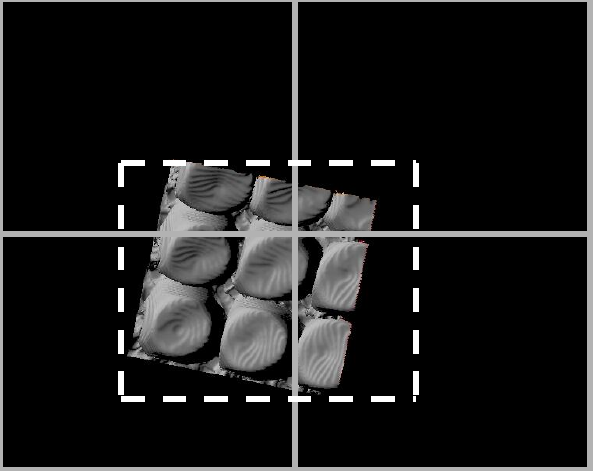
\includegraphics[width=3in]{images/FloatingViewport}
  \caption[Floating viewport.]{Even though geometry may straddle tile
    boundaries, we may be able to render it all in one pass by ``floating''
    the viewport.}
  \label{fig:FloatingViewport}
\end{figure}

Consider the geometry shown in Figure~\ref{fig:FloatingViewport} that
projects onto a screen space that fits within a single tile but is moved in
the horizontal and vertical directions so that it straddles four tiles.  If
the system limits itself to projecting onto physical tiles, the processor
must render four images even though it could generate a single
image that contains the entire geometry with the exact same pixel spacing.
Instead of rendering four tiles, \IceT can \keyterm{float} the
viewport in the global display to the space straddling the tiles.  That is,
\IceT may project the geometry to the space shown by the dotted line
in Figure~\ref{fig:FloatingViewport} and split the resulting image back
into pieces that can be displayed directly on each tile.  Hence, the system
does not need to render any polygon more than once.

When a processor's geometry fits within the floating viewport, it can cut
the rendering time dramatically.  This is most likely to happen when the
number of tiles is small compared to the number of processors and the
spatial coherency of the data is good.

The floating viewport is always enabled by default.  You can disable it by
calling \CFunc{icetDisable} with the \CEnum{ICET\_FLOATING\_VIEWPORT}
identifier.  In general, there is not much reason to turn off the floating
viewport.  The only real reason to turn off the floating viewport is to
prevent \IceT from changing the perspective matrix when in single tile
mode.  However, \IceT will change the perspective matrix anyway when
rendering with more than one tile, so any application that might render to
a tiled display should simply leave the floating viewport option on.

\index{floating~viewport|)}

\section{Active-Pixel Encoding}
\label{sec:Customizing_Compositing:Active_Pixel_Encoding}
\index{active-pixel~encoding|(}

Because each processor renders only a fraction of the total geometry, the
geometry often occupies only a fraction of the screen space in some or all
of the tiles in which it lies.  Consequently, the initial images
distributed between processors at the beginning of composition often have a
significant amount of blank space within them.  Explicitly sending this
data between processors is a waste of bandwidth.  Transferring
sparse image data rather than full image data is a well-known way to reduce
network overhead.  So far, our best method to do this has been with
active-pixel encoding.

Active-pixel encoding is a form of run-length encoding.  A traditional
run-length encoding groups pixels into contiguous groups where the color
or depth does not change.  However, in a practical 3D rendering, both
the color and depth change almost everywhere except in the background areas
where nothing is rendered.  To take advantage of this, images are grouped
into alternating run lengths of \keyterm{active pixels}, pixels that
contain geometry information, and \keyterm{inactive pixels}, pixels that
have no geometry drawn on them.  The active-pixel run length is followed by
pairs of color and depth values (or just one of the two if that is the only
data available).  The inactive pixels are not accompanied by any color or
depth information.  The depth information is assumed to be of maximum
depth, and the color values are ignored since they contain no geometry
information.

There are many other ways to encode sparse images and reduce data
redundancy.  However, we are particularly enamored with our active-pixel
encoding for this application because it exhibits all of the following
properties:

\begin{description}
\item[Fast encoding]  Image encoding requires each pixel to be visited
  exactly once.  Each visit includes a single alpha or depth comparison, a
  single addition, and at most one copy.
\item[Free decoding]  Processors typically perform a compositing as
  soon as they receive incoming data.  The compositing can be done
  directly against an image that is still encoded in sparse form.  In fact,
  the compositing can skip the comparisons for the inactive pixels.
  Thus doing compositing against encoded images is often faster than
  against unencoded images.
\item[Effective compression]  During the early stages of composition when
  the most image data must be transferred, the sparse data is commonly less
  than one fifth the size of the original data.
\item[Good worst case behavior] No image will ever grow by more than a few
  bytes of header information.  Images that have geometry drawn on every
  pixel will only have one run length.  Even images that alternate between
  active and inactive status for every pixel, and hence have a run length
  for every pixel, do not grow when encoded.  The number of bytes required
  to record two run lengths, which are stored as 16-bit integers each, is
  no more than the number of bytes saved by not recording either color or
  depth data for a single inactive pixel, which is at least 32-bits.  Thus,
  there is no penalty for recording run lengths of size one.
\end{description}

Active-pixel encoding is performed automatically during the compositing
process.  There is currently no way to turn it off.

\index{active-pixel~encoding|)}

\section{Data Replication}
\label{sec:Customizing_Compositing:Data_Replication}
\index{data~replication|(}

The primary advantage of \IceT's parallel rendering algorithms, and
sort-last rendering algorithms in general, is that they are very scalable
with respect to the size of the input geometry.  That is, there is no
overhead to adding more geometry other than the time it takes hardware to
render and there is only a logarithmic overhead for adding processors to
the job.

The down side of a sort-last approach is that the image compositing
overhead must be incurred regardless of how little geometry is being
rendered.  This overhead limits the maximum frame rate that can be achieved
by the parallel rendering.  Consequently, the parallel rendering can
potentially be slower than the serial rendering if the amount of geometry
being rendered is small.

One possible way to get higher frame rates with smaller geometries would be
to switch to a different parallel rendering mode, but doing so is
unnecessarily complicated.  Another possibility is to collect the data on
a single process and circumvent the \IceT library entirely.  This approach
is fine when using single tile mode where the image is displayed at a
single location, but is not at all straightforward when displaying to a
tiled display.

\IceT provides a better solution than either of the previous two
approaches.  If the image compositing work is dominating the rendering
time, you can set up a \keyterm{data replication group}.  To set up a data
replication group, you partition the geometry using fewer partitions than
processes, and then you share each partition with multiple processes.  The
processes that share a data partition are a replication group.  \IceT will
divide the compositing work for each replication group amongst the
processes in the group.  In essence, you are adding geometry rendering work
to remove image compositing work.

One of the most common uses for data replication groups is to simply
replicate the same geometry on all processes.  This is helpful, for
example, if your application supports lower levels of detail for
interaction.  The lower level of detail can be replicated on all
processes.  However, you could also conceivably arrange for any amount of
replication between all replicated and none replicated for a consistently
appropriate overhead as the amount of data grows.

To set up data replication groups, it is your responsibility to partition
and replicate geometry.  (\IceT knows nothing about geometry.)  You then
report what the data replication groups are with the
\CFunc{icetDataReplicationGroup} function.

\begin{Table}{3}
  \textC{void }\CFunc{icetDataReplicationGroup}\textC{(}&\textC{IceTInt}&\CArg{size}\textC{,} \\
  &\textC{const IceTInt *}&\CArg{processes}\quad\textC{);}
\end{Table}

\CFunc{icetDataReplicationGroup} simply takes an array defining the
replication group that the local process belongs to.  It is important to
ensure that all processes belonging to a group provide the same array to
\CFunc{icetDataReplicationGroup}.  As a convenience, \IceT also provides
the \CFunc{icetDataReplicationGroupColor} function that allows you to
define the data replication groups by assigning an identifier (i.e. color)
to each partition and having each process report the partition color in
which it belongs.
\begin{Table}{3}
  \textC{void }\CFunc{icetDataReplicationGroupColor}\textC{(}&\textC{IceTInt}&\CArg{color}\quad\textC{);}
\end{Table}

As an example, let us say that processes 0--3 share the same geometry, 4--7
share the same geometry, 8--11 share the same geometry, and so on.  These
replication groups could be reported with the following call (where
\textC{rank} is the local process id as stored in the \CEnum{ICET\_RANK}
state variable).
\begin{code}
icetDataReplicationGroupColor(rank/4);
\end{code}

The data replication group is stored in the
\CEnum{ICET\_DATA\_REPLICATION\_GROUP} state variable (retrievable with
\CFunc{icetGet}).  The length of the group array is stored in
\CEnum{ICET\_DATA\_REPLICATION\_GROUP\_SIZE}.  The data replication group
array is available regardless of whether you used
\CFunc{icetDataReplicationGroup} or \CFunc{icetDataReplicationGroupColor}
to define the group.  The default value is an array with one value: the
local process.

\index{data~replication|)}

\section{Timing (and Other Metrics)}
\label{sec:Customizing_Compositing:Timing}
\index{timing|(}

Whenever \CFunc{icetDrawFrame} or \CFunc{icetGLDrawFrame} is called, \IceT
measures the amount of time spent in the various tasks required for
parallel rendering.  These timings are stored in the \IceT state and can be
retrieved with \CFunc{icetGet}.  The state variables containing these
timing metrics (in seconds) are as follows.

\begin{Description}[xxxxxxxx]
\item[\CEnum{ICET\_RENDER\_TIME}] The total time spent in the drawing
  callback during the last call to \CFunc{icetDrawFrame} or
  \CFunc{icetGLDrawFrame}.
\item[\CEnum{ICET\_BUFFER\_READ\_TIME}] The total time spent copying buffer
  data and reading from \OpenGL buffers during the last call to
  \CFunc{icetDrawFrame} or \CFunc{icetGLDrawFrame}.
\item[\CEnum{ICET\_BUFFER\_WRITE\_TIME}] The total time spent writing to
  OpenGL buffers during the last call to \CFunc{icetGLDrawFrame}.  Always
  set to 0.0 after a call to \CFunc{icetDrawFrame}.
\item[\CEnum{ICET\_COMPRESS\_TIME}] The total time spent in compressing
  image data using active pixel encoding during the last call to
  \CFunc{icetDrawFrame} or \CFunc{icetGLDrawFrame}.
\item[\CEnum{ICET\_BLEND\_TIME}]/\CEnum{ICET\_COMPARE\_TIME} The total time
  spent in performing Z comparisons or color blending of images during the
  last call to \CFunc{icetDrawFrame} or \CFunc{icetGLDrawFrame}.  These two
  variables always return the same value.
\item[\CEnum{ICET\_TOTAL\_DRAW\_TIME}] The total time spent in the drawing
  callback during the last call to \CFunc{icetDrawFrame} or
  \CFunc{icetGLDrawFrame}.
\item[\CEnum{ICET\_COMPOSITE\_TIME}] The total time spent in compositing
  during the last call to \CFunc{icetDrawFrame} or \CFunc{icetGLDrawFrame}.
  Equal to $\CEnum{ICET\_TOTAL\_DRAW\_TIME} - \CEnum{ICET\_RENDER\_TIME} -
  \CEnum{ICET\_BUFFER\_READ\_TIME} - \CEnum{ICET\_BUFFER\_WRITE\_TIME}$.
\end{Description}

In addition to timing how long rendering and compositing takes, \IceT also
keeps track of how much data is transmitted during compositing.  The state
variable \CEnum{ICET\_BYTES\_SENT} stores the total number of bytes sent by
the calling process for transferring image data during the last call to
\CFunc{icetDrawFrame}.  Obviously, each process could have a different
value for \CEnum{ICET\_BYTES\_SENT}.

\IceT also keeps track of the number of times \CFunc{icetDrawFrame} or
\CFunc{icetGLDrawFrame} has been called.  This number is stored in
\CEnum{ICET\_FRAME\_COUNT}.

\index{timing|)}


% -*- latex -*-


\chapter{Strategies}
\label{chap:Strategies}

\index{strategy|(}

\IceT contains several parallel image compositing algorithms.  The type of
compositing algorithm to use is selected by choosing a
\index{strategy}\keyterm{strategy}.  This chapter describes the underlying
algorithm of each strategy.  This user's guide will give qualitative
comparisons between the strategies, but for a more quantitative analysis,
see the following paper.

\begin{quote}
  Kenneth Moreland, Brian Wylie, and Constantine Pavlakos.  ``Sort-last
  parallel rendering for viewing extremely large data sets on tile
  displays,'' In \emph{Proceedings of IEEE Symposium on Parallel and
    Large-Data Visualization and Graphics}, October 2001, pp. 85--154.
\end{quote}

A strategy is specified using the \CFunc{icetStrategy} function.

\begin{Table}{3}
  \textC{void }\CFunc{icetStrategy}\textC{(}&\textC{IceTEnum}&\CArg{strategy}\quad\textC{);}
\end{Table}

The \CArg{strategy} is set to one of the following identifiers.  A string
documenting the current strategy can be retrieved with the
\CFunc{icetGetStrategyName} function.  The following sections describe the
strategies in more detail.

% -*- latex -*-

  \begin{Description}
  \item[\CEnum{ICET\_STRATEGY\_SEQUENTIAL}]
    Basically applies a ``traditional'' single tile composition (such as
    binary swap) to each tile in the order they were defined.  Because each
    process must take part in the composition of each tile regardless of
    whether they draw into it, this strategy is usually inefficient when
    compositing for more than one tile, but is recommended for the single
    tile case because it bypasses some of the communication necessary for
    the other multi-tile strategies.
    \index{strategy!sequential}
  \item[\CEnum{ICET\_STRATEGY\_DIRECT}] As each process renders an image
    for a tile, that image is sent directly to the process that will
    display that tile.  This usually results in a few processes receiving
    and processing the majority of the data, and is therefore usually an
    inefficient strategy.
    \index{strategy!direct}
  \item[\CEnum{ICET\_STRATEGY\_SPLIT}] Like \CEnum{ICET\_STRATEGY\_DIRECT},
    except that the tiles are split up, and each process is assigned a
    piece of a tile in such a way that each process receives and handles
    about the same amount of data.  This strategy is often very efficient,
    but due to the large amount of messages passed, it has not proven to be
    very scalable or robust.
    \index{strategy!split}
  \item[\CEnum{ICET\_STRATEGY\_REDUCE}] A two phase algorithm.  In the
    first phase, tile images are redistributed such that each process has
    one image for one tile.  In the second phase, a ``traditional'' single
    tile composition is performed for each tile.  Since each process
    contains an image for only one tile, all these compositions may happen
    simultaneously.  This is a well rounded strategy that seems to perform
    well in a wide variety of multi-tile applications.  (However, in the
    special case where only one tile is defined, the sequential strategy is
    probably better.)
    \index{strategy!reduce}
  \item[\CEnum{ICET\_STRATEGY\_VTREE}] An extension to the binary tree
    algorithm for image composition.  Sets up a ``virtual'' composition
    tree for each tile image.  Processes that belong to multiple trees
    (because they render to more than one tile) are allowed to float
    between trees.  This strategy is not quite as well load balanced as
    \CEnum{ICET\_STRATEGY\_REDUCE} or \CEnum{ICET\_STRATEGY\_SPLIT}, but
    has very well behaved network communication.
    \index{strategy!virtual~trees}
  \end{Description}


To describe the \IceT compositing algorithms, we will use the example
parallel rendering problem shown in Figure~\ref{fig:ExampleInputs} where 6
processes are each rendering their own piece of a shuttle model to a two
tile display.

\begin{figure}
  \centering
  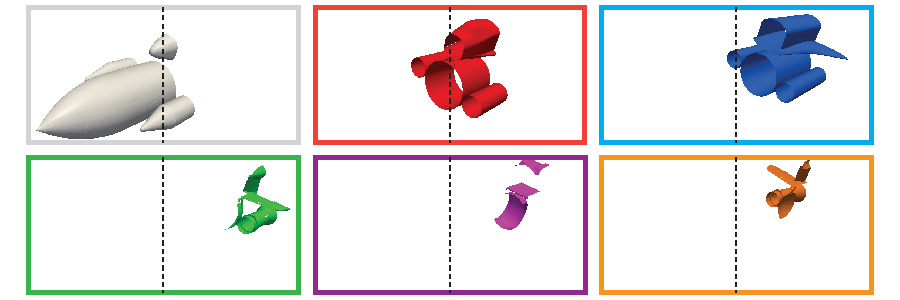
\includegraphics{images/AllInput}
  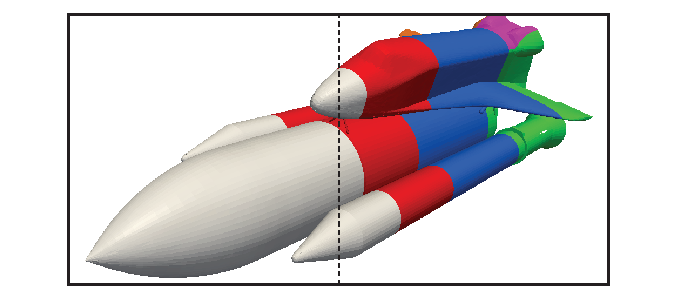
\includegraphics{images/CompositedInput}
  \caption[Example compositing problem.]{An example of six processes
    rendering to two tiles (top) and their composited image (bottom).}
  \label{fig:ExampleInputs}
\end{figure}

In this example, processes are denoted, in no particular order, by the
colors gray, red, blue, green, purple, and orange.  The colors of the
geometry correspond to the process that generated each piece.  Image
boarder colors denote the process that generates and holds that image.
(Apologies to those having troubles resolving the colors due to poor
display, printout, or vision deficiencies.  It should not be hard to follow the
descriptions either way.)

\section{Single Image Compositing}
\label{sec:Strategies:SingleImageCompositing}

\index{single~image~composite|(}
\index{compositing!single~image|(}

Before discussing the multi-tile image compositing algorithms implemented
by \IceT, we visit the standard single image compositing algorithms.  You
cannot directly use a single image compositing algorithm as a strategy
(most of the multi-tile algorithms work well in ``single-tile'' mode), but
these compositing algorithms are used as ``subroutines'' in some of the
multi-tile algorithms.  A reference to a
\index{single~image~composite~network}\keyterm{single image composite
  network} in the subsequent compositing algorithm descriptions refers to
the algorithms described here.

You can, however, choose which single image strategy is used by the main
multi-tile strategy.  This is selected with the
\CFunc{icetSingleImageStrategy} function.

\begin{Table}{3}
  \textC{void }\CFunc{icetSingleImageStrategy}\textC{(}&\textC{IceTEnum}&\CArg{strategy}\quad\textC{);}
\end{Table}

The \CArg{strategy} is set to one of the following enumerations.  A string
documenting the current strategy can be retrieved with the
\CFunc{icetGetSingleImageStrategyName} function.  The following sections
describe the single image strategies in more detail.

% -*- latex -*-

\begin{Description}
\item[\CEnum{ICET\_SINGLE\_IMAGE\_STRATEGY\_AUTOMATIC}] Automatically
  chooses which single image strategy to use based on the number of
  processes participating in the composition.
  \index{single~image~strategy!automatic}
\item[\CEnum{ICET\_SINGLE\_IMAGE\_STRATEGY\_BSWAP}] The classic binary swap
  compositing algorithm.  At each phase of the algorithm, each process
  partners with another, sends half of its image to its partner, and
  receives the opposite half from its partner.  The processes are then
  partitioned into two groups that each have the same image part, and the
  algorithm recurses.
  \index{single~image~strategy!binary~swap}
\item[\CEnum{ICET\_SINGLE\_IMAGE\_STRATEGY\_TREE}] At each phase, each
  process partners with another, and one of the processes sends its entire
  image to the other.  The algorithm recurses with the group of processes
  that received images until only one process has an image.
  \index{single~image~strategy!tree}
\end{Description}


\subsection{Tree Compositing}

\index{compositing!tree|(}
\index{tree~composite|(}
\index{binary~tree~composite|(}

The \keyterm{tree composite} algorithm (sometimes also called binary tree
composite due to its pair-wise grouping) is a simple algorithm that
iteratively combines full images together until they are all merged into a
single image.  The tree composite sub-strategy is selected by calling
\CFunc{icetSingleImageStrategy} with
\CEnum{ICET\_SINGLE\_IMAGE\_STRATEGY\_TREE}.  The basic network for tree
composite is shown in Figure~\ref{fig:BinaryTree}.

\begin{figure}
  \centering
  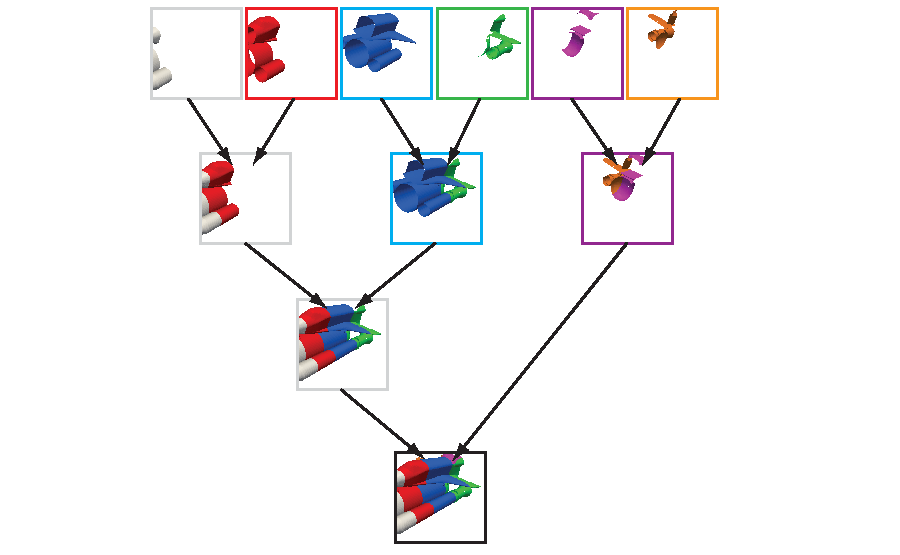
\includegraphics{images/BinaryTree}
  \caption[Tree composite network.]{Tree composite network.  Arrows
    represent the passing of data from one stage to the next.  Processes
    receiving multiple images composite them together.}
  \label{fig:BinaryTree}
\end{figure}

The tree compositing algorithm is organized in stages.  At each stage the
processes pair up.  One of the processes sends its data to its pair and
then drops out of the computation.  The receiving process combines the two
images (using the \index{compositing~operation}compositing operation
described in
Chapter~\ref{sec:Customizing_Compositing:Compositing_Operation}) and
continues to the next stage.  Processing continues until there is only one
image (and one process) remaining.

As just defined, the tree composite algorithm only handles process counts
that are a power of two (that is, the number of processes is equal to $2^i$
for some integer $i$).  \IceT handles non-powers of two gracefully.  At any
stage where the number of processes is not even and one of the processes
cannot be paired, that leftover process does nothing for that stage but
then continues to participate in the next stage.  An example of this can be
seen in the second stage of Figure~\ref{fig:BinaryTree}.

The advantages of tree composite are its regular and efficient data
transfers.  The limiting factor of tree compositing is that at each stage
of the algorithm half of the processes drop out of the computation.  Thus,
for more than a few processes tree compositing provides poor process
utilization.

\index{binary~tree~composite|)}
\index{tree~composite|)}
\index{compositing!tree|)}

\subsection{Binary-Swap Compositing}

\index{compositing!binary~swap|(}
\index{binary~swap~composite|(}

The second single image compositing algorithm provided by \IceT is the
\keyterm{binary-swap} algorithm.  The binary-swap composite sub-strategy is
selected by calling \CFunc{icetSingleImageStrategy} with
\CEnum{ICET\_SINGLE\_IMAGE\_STRATEGY\_BINARY\_SWAP}.  The basic network for
binary-swap composite is shown in Figure~\ref{fig:BinarySwap}

\begin{figure}
  \centering
  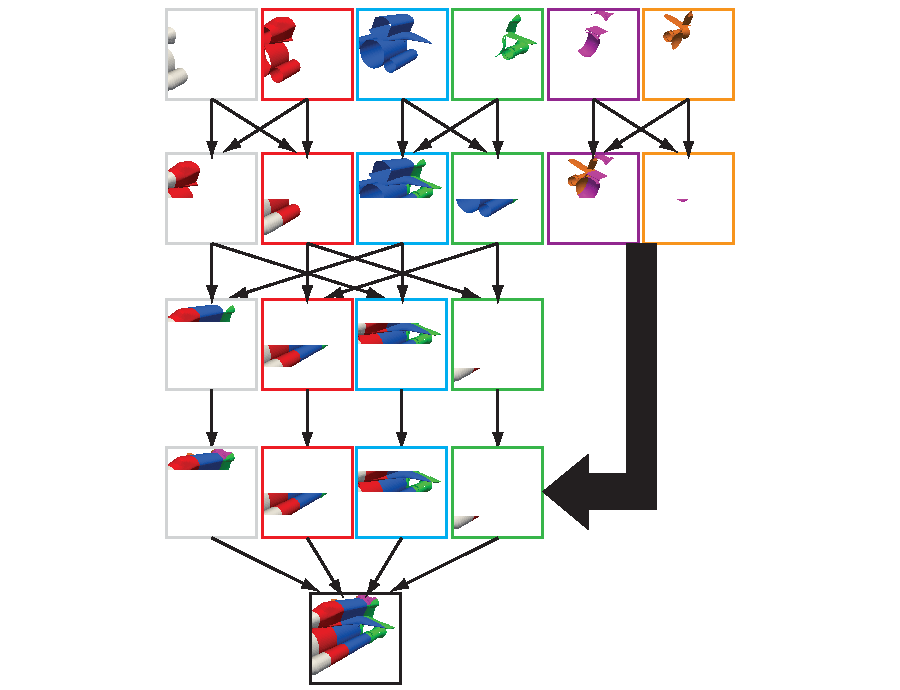
\includegraphics{images/BinarySwap}
  \caption[Binary-swap composite network.]{Binary-swap composite network.
    Arrows represent the passing of data from one stage to the next.
    Processes receiving multiple images composite or stitch them together.
    At most stages each process divides its image data and distributes it.
    The distribution of image data can be inferred from the target images.}
  \label{fig:BinarySwap}
\end{figure}

Like tree compositing, binary swap is organized in stages, and at each
stage the processes pair up.  However, rather than have one process send
all the data to the other, the image space is divided in two and the
processes swap image data so that each process has all the data for part of
the image.  At the next stage, the processes pair up again, but with
different partners that have the same partition of the image.  Processing
continues until each of the $N$ processes have an image $1/N$ the size of
the original image.  At this point, all the processes send their sub-image
to the display processes where the images are stitched together.

As just defined, the binary-swap composite algorithm only handles processes
that are a power of two (that is, the number of processes is equal to $2^i$
for some integer $i$).  Some binary-swap implementations handle non-powers
of two by reducing the problem to the next largest power of two and
dropping the leftover processes, but \IceT handles non-powers of two more
gracefully than that.  Instead, \IceT first finds the largest group of
processes that is a power of two, makes a partition out of them, then finds
the next largest group of processes that remain that is a power of two,
makes a partition out of them, and so on.  Each partition runs binary-swap
independently up to the point where each process has its own piece of data.
At this point, the smaller partitions send their image data to processes of
the larger partitions, dividing up images where necessary.  The largest
partition then finishes the compositing in the normal way by collecting all
of the pieces.

An example of compositing with a non-power of two is given in
Figure~\ref{fig:BinarySwap}.  The six processes are partitioned first into
a group of 4 and then into a group of 2.  After swapping, the processes in
the smaller group send images to the larger group.  In this case, the purple
process sends image data to the gray and blue processes, and the orange
process sends to the red and green processes.

Like tree composite, binary swap exhibits regular and efficient data
transfers.  In addition, binary swap involves the use of all the processes
throughout most of the compositing.  Consequently, binary swap exhibits
very good process utilization and scaling with respect to the number of
processes on which it is run.

The most inefficient part of binary swap is the collection of image
fragments at the end, which is an extra step that tree composite does not
need to take.  Most of the time the better parallel efficiency of binary
swap over tree composite more than compensates for the extra collection
step.

\index{binary~swap~composite|)}
\index{compositing!binary~swap|)}

\subsection{Automatic Algorithm Selection}

\index{automatic~composite~selection|(}
\index{compositing!automatic~selection|(}

\IceT also supports the automatic selection of the single image
sub-strategy.  This automatic selection is enabled by calling
\CFunc{icetSingleImageStrategy} with
\CEnum{ICET\_SINGLE\_IMAGE\_STRATEGY\_AUTOMATIC}. (It is also the default
for the single image strategy.)

The automatic selection attempts to guess at the best strategy.  The
intension is that \IceT can internally pick the best strategy depending on
how the compositing is being used.  For example, through some empirical
studies, we found that the binary tree algorithm was more efficient than
binary swap on less then 8 processes and less efficient on more than 8
processes.  Consequently, \IceT automatically switches between the two
algorithms based on the amount of processes involved in the compositing.

\index{compositing!automatic~selection|)}
\index{automatic~composite~selection|)}

\subsection{Ordered Compositing}

\index{compositing!ordered|(}

In some applications, the order in which images are composited together
makes a difference (see the Volume Rendering section in
Chapter~\ref{sec:Customizing_Compositing:Volume_Rendering}).  The details
on how ordered compositing is achieved is not given here, but the basic
idea for both compositing algorithms is that they first swizzle the
processes so that their order matches the order in which the images need to
be composited together.  When compositing images together, they make sure
to maintain over/under constancy based on the swizzled ranks from the
originating processes.  The networks are also managed such that no two
images are composited that are not directly ``next'' to each other (that
is, there is no image that needs to be inserted between them).

\index{compositing!ordered|)}

\index{compositing!single~image|)}
\index{single~image~composite|)}

\section{Reduce Strategy}
\label{sec:Strategies:Reduce}

\index{strategy!reduce|(}
\index{reduce~strategy|see{strategy, reduce}}
\index{reduce~to~single~tile|see{strategy, reduce}}

An effective strategy implemented in \IceT is the \keyterm{reduce to single
  tile strategy} (or simply the reduce strategy).  In this strategy, the
multi-tile composite problem is efficiently reduced to a set of single
image compositing problems, which are well studied and discussed in the
previous section.  The reduce strategy is selected by calling
\CFunc{icetStrategy} with the \CEnum{ICET\_STRATEGY\_REDUCE} argument.

\begin{figure}
  \centering
  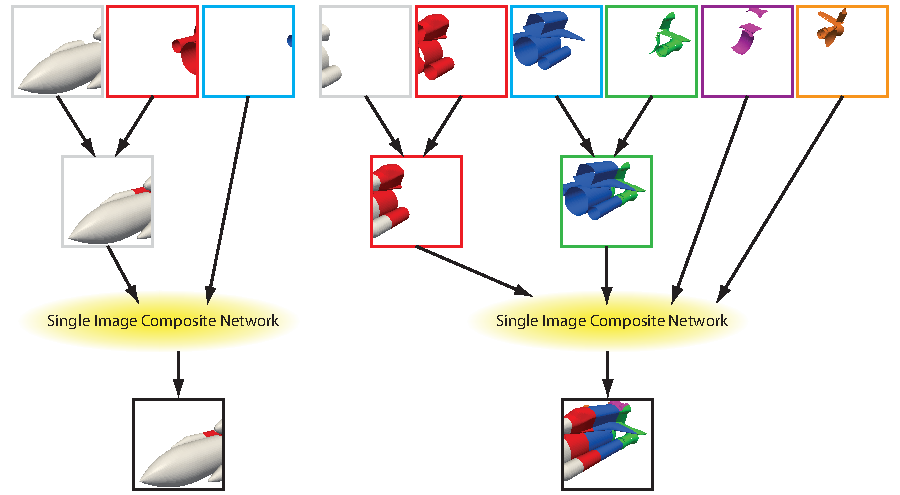
\includegraphics{images/ReduceComposite}
  \caption[Reduce strategy composite network.]{Composite network for reduce
    strategy.  Arrows represent the passing of data from one stage to the
    next.  Processes receiving multiple images composite them together.
    The single image composite network is described in a preceding
    section.}
  \label{fig:ReduceComposite}
\end{figure}

The reduce strategy is performed in two phases.  In the first phase,
processes are partitioned into groups, each of which is responsible for
compositing the image of one of the tiles.  The number of processes
assigned to each tile is proportional to the number of non-empty images
rendered for the corresponding tile.  In the example shown in
Figure~\ref{fig:ReduceComposite} there are a total of 9 non-empty images.
The left tile has 3 of the 9, that is $\frac{1}{3}$, of the images and thus
is assigned $\frac{1}{3} \times 6 = 2$ processes.  Likewise, the right
image is assigned $\frac{2}{3} \times 6 = 4$ processes.

When assigning processes to tiles, display processes and processes rendering
images to the tile are given preference.  In the example of
Figure~\ref{fig:ReduceComposite}, the gray and blue processes are assigned
to the left tile.  The remainder are assigned to the right tile.  Any image
generated by a process that does not belong to the destination tile is
transferred to a process assigned to the tile.  In the example, the three
processes that render two images, gray, red, and blue, each pass one of
their images to a process in the opposing process group.  All of these
transfers have unique senders and receivers and thus can happen
simultaneously.

In the second phase of the reduce strategy, each group of processes
independently composites its images together using one of the single image
compositing algorithms described in the preceding section.

The reduce strategy supports ordered compositing.  It does this by ensuring
in the first phase that processes receive only images that are ``near'' the
image they hold, that is, there is no other image in between the two images
in the visibility ordering.  The single image compositing algorithms of the
second phase each support their own ordered compositing.

\index{strategy!reduce|)}

\section{Split Strategy}
\label{sec:Strategies:Split}

\index{strategy!split|(}
\index{split~strategy|see{strategy, split}}
\index{tile~split~and~delegate|see{strategy, split}}

The \keyterm{tile split and delegate strategy} (or simply the split
strategy) is a simple algorithm that splits up tiles, assigns each piece to
a process, and then sends image fragments directly to the processes for
compositing.  The split strategy makes efficient use of processing
resources, but exhibits haphazard and copious message passing which can
cause issues on some high speed interconnects.  The split strategy is
selected by calling \CFunc{icetStrategy} with the
\CEnum{ICET\_STRATEGY\_SPLIT} argument.

\begin{figure}
  \centering
  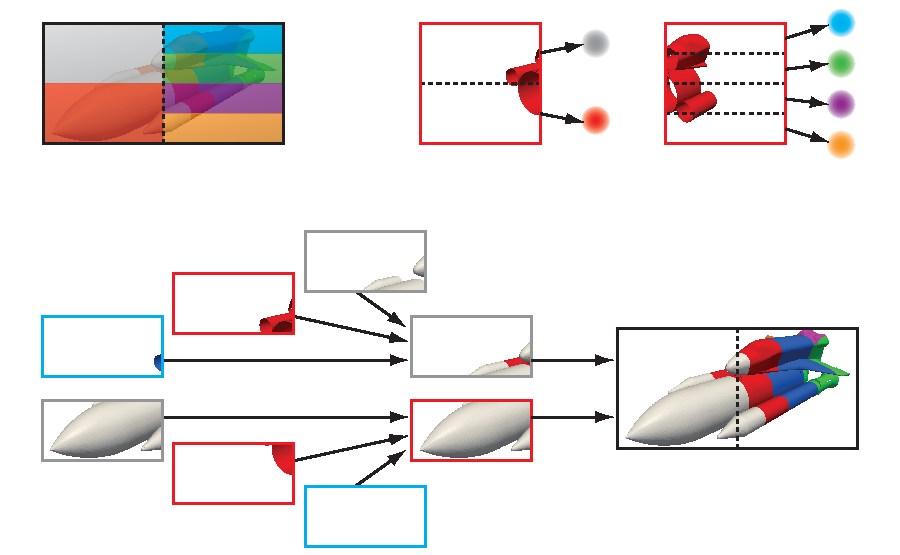
\includegraphics{images/TileSplit}
  \caption[Split strategy composite network.]{Compositing for split
    strategy.  First tiles are split and assigned to processes (upper
    left).  Then each process simultaneously sends its images to the
    responsible process (upper right) and receives all sub-images for its
    piece (bottom).  The composited pieces are then collected and stitched
    together.}
  \label{fig:TileSplit}
\end{figure}

The split strategy first assigns processes to tiles similar to how they are
assigned in the reduce strategy described previously.  That is, the number
of processes per tile is proportional to the number of non-empty images
generated for it.  Each tile is then split up evenly amongst all processes
assigned to it.  In the example in Figure~\ref{fig:TileSplit}, the upper
left image shows that the left image is split between 2 processes and the
right image is split amongst 4 processes.

On being assigned a section of tile, each process prepares to receive data
from all the sending processes using asynchronous receives.  Each process
then renders its images, splits them up, and sends the sub-images to the
corresponding process.  When a process is ready and as it receives data,
the incoming images are composited together.  Once all of the incoming
images are composited, the complete sub-image is sent to the display process
to be stitched together.

The split strategy does not support ordered compositing.  Using the split
strategy in color blending mode will fail.

\index{strategy!split|)}

\section{Virtual Trees Strategy}
\label{sec:Strategies:Vertial_Trees}

\index{strategy!virtual~trees|(}
\index{virtual~trees|see{strategy, virtual trees}}

The \keyterm{virtual trees strategy} is based on the binary tree
compositing algorithm, but performs multiple composites simultaneously to
regain some of the load balance lost in the original algorithm.  The
virtual trees strategy has nice regular communications, but still suffers
from some load imbalance, particularly when using fewer tiles and in later
stages of the algorithm.  The virtual trees strategy is selected by calling
\CFunc{icetStrategy} with the \CEnum{ICET\_STRATEGY\_VTREE} argument.

\begin{figure}
  \centering
  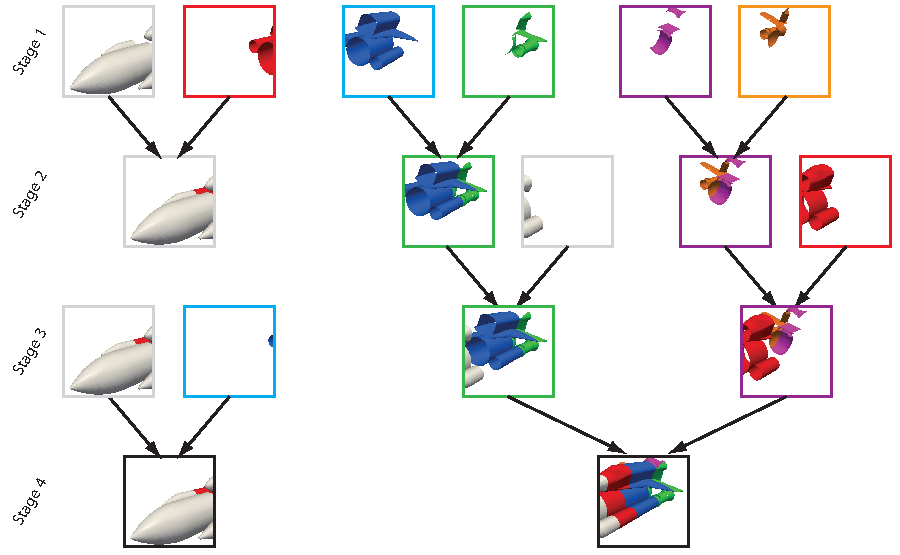
\includegraphics{images/VTrees}
  \caption[Virtual trees composite network.]{Composite network for virtual
    trees strategy.  Arrows represent the passing of data from one state to
    the next.  Processes receiving multiple images composite them
    together.}
  \label{fig:VTreesComposite}
\end{figure}

The virtual trees strategy works by creating a ``virtual'' tree for each
tile.  Contained in each tree are processes that have rendered an image for
that display tile.  The algorithm proceeds much like the binary tree
composition algorithm except that the processes float amongst the trees,
helping with the compositing as they become available.
Figure~\ref{fig:VTreesComposite} shows an example of the virtual trees
compositing.  In particular, notice that the gray process takes part in the
left tree in stage 1, then floats to take part in the right tree in stage
2, and then returns to take part in the left tree in stage 3.

When necessary, the process must keep track of multiple images belonging to
different virtual trees.  Two conserve memory, images are not rendered
until they are needed.  Also, a process can only hold two images at a time:
one that it is sending and one that it is receiving.  If a process is
holding an image for one tile, it cannot receive an image for another tile
until it sends away the image it is holding.

The virtual trees strategy does not support ordered compositing.  Using the
virtual trees strategy in color blending mode will fail.

\index{strategy!virtual~trees|)}

\section{Sequential Strategy}
\label{sec:Strategies:Sequential}

\index{strategy!sequential|(}
\index{sequential~strategy|see{strategy, sequential}}

The \keyterm{sequential strategy} sequentially addresses the tiles, but
performs parallel compositing for each tile.  The sequential strategy is
selected by calling \CFunc{icetStrategy} with the
\CEnum{ICET\_STRATEGY\_SEQUENTIAL} argument.

\begin{figure}
  \centering
  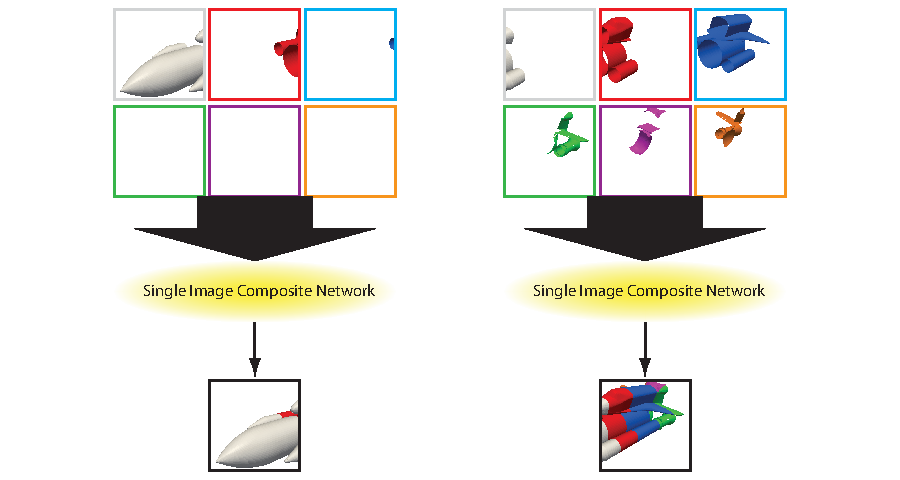
\includegraphics{images/SequentialComposite}
  \caption[Sequential compositing network.]{Composite network for
    sequential compositing.  One at a time, each tile is composited using a
    parallel single image composite network described in a previous
    section.}
  \label{fig:SequentialComposite}
\end{figure}

The sequential strategy iterates over all of the tiles.  For each tile, it
composites all the images for that tile using one of the single image
compositing algorithms described in that preceding section.  As
demonstrated in the example in Figure~\ref{fig:SequentialComposite}, images
from all processes are composited for each tile regardless of whether some
of them may be empty.

Since the single image compositing algorithms support ordered
compositing, the sequential strategy also supports ordered compositing.

The sequential strategy is really only implemented as a baseline algorithm to
compare other algorithms.  In general, the reduce strategy does at least as
well or outperforms the sequential strategy.  We have observed this even in
single tile mode, possibly because the reduce strategy can throw away empty
images.

\index{strategy!sequential|)}

\section{Direct Send Strategy}
\label{sec:Strategies:DirectSend}

\index{strategy!direct~send|(}
\index{direct~send~strategy|see{strategy, direct send}}

The \keyterm{direct send strategy} is the simplest of all the strategies.
Each process simply renders its images and sends them directly to the
display process where the images get composited, as shown in
Figure~\ref{fig:DirectSend}.  The direct send strategy is selected by
calling \CFunc{icetStrategy} with the \CEnum{ICET\_STRATEGY\_DIRECT}
argument.

\begin{figure}
  \centering
  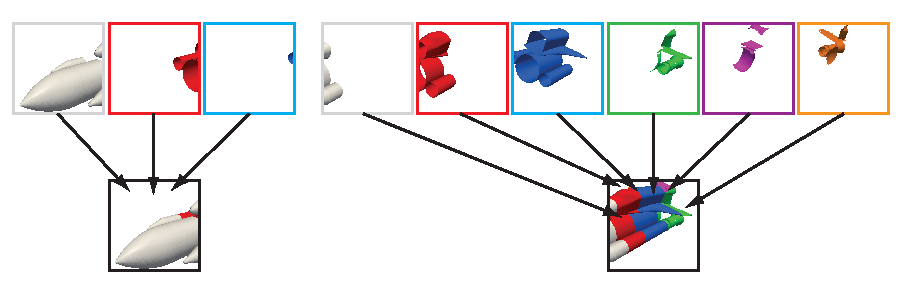
\includegraphics{images/DirectSend}
  \caption[Direct send compositing network.]{Composite network for direct
    send compositing.  Arrows represent the passing of data from one
    process to another.  Receiving process composite all incoming images
    together.}
  \label{fig:DirectSend}
\end{figure}

The direct send strategy is usually a poor performer.  It was designed as a
low watermark to compare to other compositing strategies.  The direct send
strategy does, however, support ordered compositing.

\index{strategy!direct~send|)}

\section{Implementing New Strategies}

The \IceT API was written while its strategies were being developed.  As
such, the design yields for the relatively simplistic addition of both new
multi-tile strategies and new single-image strategies.  This section will
provide the basic overview of how to add a new strategy.  It is probably
easiest to start by modifying your \IceT source to insert your own strategy
in the \textC{src/strategies} directory of the \IceT source distribution.

A strategy in \IceT is created by simply defining a function that performs
the operation.  A multi-tile strategy (one selected with
\CFunc{icetStrategy}) should take no arguments and return an
\CType{IceTImage}.  Thus, a new multi-tile strategy function would look
something like this.  (The following sections will provide details on
performing the individual tasks of the implementation.)

\begin{code}
IceTImage icetCustomMultiTileCompose(void)
{
    /* Render images. */
    /* Transfer data. */
    /* Composite pixels. */
    /* Store results in image. */
    return image;
}
\end{code}

To expose the strategy from the \IceT interface, add an identifier to
\textC{IceT.h} starting with \textC{ICET\_STRATEGY\_} to the list of
existing strategy identifiers.  Then modify the functions in
\textC{src/strategies/select.c} to expose this new identifier to the rest
of the \IceT library.  In particular, add your new identifier to the switch
statements in the following functions.

\begin{description}
\item[\CFunc{icetStrategyValid}] Simply add your identifier to the list so
  that \IceT can verify that your strategy is defined.
\item[\CFunc{icetStrategyNameFromEnum}] Add a short human-readable name for
  your strategy.  This is the string returned from
  \CFunc{icetGetStrategyName}.
\item[\CFunc{icetStrategySupportsOrder}] Return \CEnum{ICET\_TRUE} if your
  strategy can properly composite based on the ordering given in
  \CEnum{ICET\_COMPOSITE\_ORDER}.  Return \CEnum{ICET\_FALSE} otherwise.
  This value gets stored in the
  \CEnum{ICET\_STRATEGY\_SUPPORTS\_ORDERING}.
\item[\CFunc{icetInvokeStrategy}] Call the function that invokes your
  strategy's image compositing (\textC{icetCustomMultiTileCompose} in the
  example above).
\end{description}

The process for creating a single-image strategy (one selected with
\CFunc{icetSingleImageStrategy} is similar.  The first step is define a
function that performs the compositing.  However, the single-image
composite function takes arguments that define the image to composite and
the group of processes contributing.  A new single-image strategy function
would look something like this.

\begin{code}
void icetCustomSingleImageCompose(IceTInt *compose_group, IceTInt group_size,
                                  IceTInt image_dest,
                                  IceTImage image)
{
    /* Transfer data. */
    /* Composite pixels. */
    /* Store results in image. */
}
\end{code}

The first argument, \CArg{compose\_group}, is an array of process ranks.
The pixels are to be composited in the order specified in this array.  The
second argument, \CArg{group\_size}, specifies how many processes are
contributing to the image and also specifies the length of
\CArg{compose\_group}.  The third argument, \CArg{image\_dest}, specifies
the process in which the final composed image should be placed.  It is an
index into \CArg{compose\_group}, not the actual rank of the process.  The
final argument, \CArg{image} contains the input images to be composited
together.  It is also used to store the results of the compositing.  The
process with rank \textC{\CArg{compose\_group}[\CArg{image\_dest}]} fills
\CArg{image} with the resulting composited image.

To expose the single-image strategy from the \IceT interface, add an
identifier to \textC{IceT.h} starting with
\textC{ICET\_SINGLE\_IMAGE\_STRATEGY\_} to the list of existing
single-image strategy identifiers.  Then modify the functions in
\textC{src/strategies/select.c} to expose this new identifier to the rest
of the \IceT library.  In particular, add your new identifier to the switch
statements in the following functions.

\begin{description}
\item[\CFunc{icetSingleImageStrategyValid}] Simply add your identifier to
  the list so that \IceT can verify that your strategy is defined.
\item[\CFunc{icetSingleImageStrategyNameFromEnum}] Add a short
  human-readable name for your strategy.  This is the string returned from
  \CFunc{icetGetSingleImageStrategyName}.
\item[\CFunc{icetInvokeSingleImageStrategy}] Call the function that invokes
  your strategy's image compositing (\textC{icetCustomSingleImageCompose}
  in the example above).
\end{description}

\subsection{Internal State Variables for Compositing}

The strategy compose functions are expected to get many of its parameters
and other relevant information from the \IceT state.  Many of the relevant
state variables are described in the documentation for the \CFunc{icetGet}
functions (as well as elsewhere throughout this document).  There are also
several ``hidden'' state variables for internal use.  The ones specifically
useful for within a composite function are listed here (along with the
variable type, number of entries, and a description).  Note that these
state variables generally should be read from, not written to.

\begin{Description}[xxxxxxxx]
\item[\CEnum{ICET\_ALL\_CONTAINED\_TILES\_MASKS}] (boolean,
  \CEnum{ICET\_NUM\_TILES} $\times$ \CEnum{ICET\_NUM\_PROCESSES}) Contains
  an appended list of \CEnum{ICET\_CONTAINED\_TILES\_MASK} variables for
  all processes.  Given process $p$ and tile $t$, the entry at
  $p+\CEnum{ICET\_NUM\_TILES} \times t$ contains the flag describing
  whether process $p$ renders a non-blank image for tile $t$.  This
  variable is the same on all processes.
\item[\CEnum{ICET\_CONTAINED\_TILES\_LIST}] (integer,
  \CEnum{ICET\_NUM\_CONTAINED\_TILES}) All the tiles into which the local
  geometry projects.  In other words, this is the list of tiles which will
  not be empty after local rendering.  The local processor should generate
  images for these tiles and participate in the composition of them.
\item[\CEnum{ICET\_CONTAINED\_TILES\_MASK}] (boolean,
  \CEnum{ICET\_NUM\_TILES}) This is a list of boolean flags, one per tile.
  The flag is 1 if the local geometry projects onto the tile (that is, the
  local render will not be empty for that tile) and 0 otherwise.  This
  gives the same information as \CEnum{ICET\_CONTAINED\_TILES\_LIST}, but
  in a different way that can be more convenient in some circumstances.
\item[\CEnum{ICET\_CONTAINED\_VIEWPORT}] (integer, 4) Describes the region
  of the viewport that the geometry being rendered locally projects onto.
  The bounds of the data (given by \CFunc{icetBoundingBox} or
  \CFunc{icetBoundingVertices}) onto the tile display and determines the
  region of the tile display the data covers.  The values in the four-tuple
  correspond to x, y, width, and height, respectively, of the projection in
  global pixel coordinates.  This variable in conjunction with the
  \CEnum{ICET\_NEAR\_DEPTH} and \CEnum{ICET\_FAR\_DEPTH} give the full 3D
  projection of the local data in window space.
\item[\CEnum{ICET\_FAR\_DEPTH}] (double, 1) The maximum depth value of the
  local geometry after projection.  See \CEnum{ICET\_CONTAINED\_VIEWPORTS}
  for more details.
\item[\CEnum{ICET\_IS\_DRAWING\_FRAME}] (boolean, 1) Set to true while in a
  call to \CFunc{icetDrawFrame} and set to false otherwise.  This should
  always be set to true while the compose function is being executed.
\item[\CEnum{ICET\_MODELVIEW\_MATRIX}] (double, 16) The current modelview
  matrix as passed to \CFunc{icetDrawFrame} or read from OpenGL at the
  invocation of \CFunc{icetGLDrawFrame}.
\item[\CEnum{ICET\_NEAR\_DEPTH}] (double, 1) The minimum depth value of the
  local geometry after projection.  See \CEnum{ICET\_CONTAINED\_VIEWPORTS}
  for more details.
\item[\CEnum{ICET\_NUM\_CONTAINED\_TILES}] (integer, 1) The number of tiles
  into which the local geometry projects.  This is the length of the
  \CEnum{ICET\_CONTAINED\_TILES\_LIST} variable.
\item[\CEnum{ICET\_PROJECTION\_MATRIX}] (double, 16) The current projection
  matrix as passed to \CFunc{icetDrawFrame} or read from OpenGL at the
  invocation of \CFunc{icetGLDrawFrame}.
\item[\CEnum{ICET\_TILE\_CONTRIB\_COUNTS}] (integer,
  \CEnum{ICET\_NUM\_TILES}) For each tile, provides the number of processes
  that will produce a non-empty image for that tile.
\item[\CEnum{ICET\_TOTAL\_IMAGE\_COUNT}] (integer, 1) The total number of
  non-empty images produced by all processes for all tiles.  This variable
  is the sum of all entries in \CEnum{ICET\_TILE\_CONTRIB\_COUNTS}.
\end{Description}

\label{manpage:icetUnsafeStateGet}
In addition to several internal state variables, \IceT also has several
internal functions for accessing them.  The most important set for
implementing a strategy is \CFunc{icetUnsafeStateGet} suite of functions,
which are defined in the \index{IceTDevState.h}\textC{IceTDevState.h}
header file.

\begin{Table}{4}
  \textC{IceTDouble *}&\icetUnsafeStateGetDouble\textC{(}&\textC{GLenum}&\CArg{pname}\quad\textC{);} \\
  \textC{IceTFloat *}&\icetUnsafeStateGetFloat\textC{(}&\textC{GLenum}&\CArg{pname}\quad\textC{);} \\
  \textC{IceTInt *}&\icetUnsafeStateGetInteger\textC{(}&\textC{GLenum}&\CArg{pname}\quad\textC{);} \\
  \textC{IceTBoolean *}&\icetUnsafeStateGetBoolean\textC{(}&\textC{GLenum}&\CArg{pname}\quad\textC{);} \\
  \textC{IceTVoid **}&\icetUnsafeStateGetPointer\textC{(}&\textC{GLenum}&\CArg{pname}\quad\textC{);}
\end{Table}

The implementation for the \CFunc{icetGet} functions is to copy the data
into a memory buffer you provide, performing type conversion as necessary.
The \CFunc{icetUnsafeStateGet} functions simply return the internal pointer
where the data is stored.  This can be faster and more convenient (since
you do not have to allocate your own memory), but is unsafe in two ways.
First, if the state variable is changed, the pointer you receive can become
invalid.  Second, no type conversion is performed.  You have to make sure
that you request a pointer of the correct type (or you will get an error).
Since the state setting functions are hidden from the end user API, it is
possible to manage these erroneous conditions.

\subsection{Memory Management}

Compositing algorithms by their nature require buffers of memory of
non-trivial size to hold images, among other data, that are not needed in
between calls to the compositing.  One approach is to simply use the
standard C \CFuncExternal{malloc} and \CFuncExternal{free} functions.
However, some implementations of
\CFuncExternal{malloc}/\CFuncExternal{free} are not always efficient, and
even the best implementations can have a tendency to fragment memory over
time as large buffers are allocated and released.

To ensure efficient memory allocation, \IceT provides its own memory
management that is simple but effective for its compositing operations.
\IceT keeps around a pool of memory to be used by various components of the
API.  To use the \index{memory~pool}\index{pool!memory}\keyterm{memory
  pool}, the code first clears the buffer and ensures that it is big
enough.  The code then reserves sections of the pool for various buffers.
Since this pool changes size infrequently, allocating time or memory
fragmentation is not an issue.  The size of the allocated memory is also
minimized since it is shared throughout all of \IceT.

\label{manpage:icetResizeBuffer}
The \CFunc{icetResizeBuffer} function is used to clear out the memory
pool.  The declaration for this function is located in the
\index{context.h}\textC{context.h} header file.

\begin{Table}{3}
  \textC{void }\CFunc{icetResizeBuffer}\textC{(}&\textC{int}&\CArg{size}\quad\textC{);}
\end{Table}

The \CFunc{icetResizeBuffer} function ensures that the memory pool is at
least \CArg{size} bytes large.  It also resets all previously allocated
memory (that is, freeing it back into the pool).  This has two important
consequences.  First, you must know the amount of memory you need
\emph{a-priori}.  You cannot resize the buffer once you have started
allocating memory blocks.  If you try to do so, the previously allocated
blocks (potentially) will be destroyed.

Second, since this block of data is shared amongst all functions of \IceT,
you must be aware that other \IceT code can potentially release your memory
and allocate its own.  You should feel free to use \IceT's memory pool from
within the compose function of your strategy and the image that it returns
is best allocated from this buffer.  Furthermore, the helper functions
described in this section to implement your own strategy are also safe to
call.  Be aware, however, that in between calls to your composite function
the memory you allocate will be lost and you will have to reallocate your
buffers.

\label{manpage:icetReserveBufferMem}
Once you have sized the memory pool, use \CFunc{icetReserveBufferMem} to
allocate a chunk of memory.

\begin{Table}{3}
  \textC{void *}\CFunc{icetReserveBufferMem}\textC{(}&\textC{int}&\CArg{size}\quad\textC{);}
\end{Table}

\CFunc{icetReserveBufferMem} returns a pointer to a buffer reserved to the
given size.  The buffer is aligned on 64-bit boundaries to help prevent
illegal memory accesses.

The following code snippet (taken from the direct send strategy)
demonstrates the use of \CFunc{icetResizeBuffer} and
\CFunc{icetReserveBufferMem}.  (The image size functions are described in
the section on image functions.)

\begin{code}
    icetResizeBuffer(  2*icetSparseImageSize(max_pixels)
                     + icetFullImageSize(max_pixels)
                     + num_tiles*sizeof(GLint));
    inImage     = icetReserveBufferMem(icetSparseImageSize(max_pixels));
    outImage    = icetReserveBufferMem(icetSparseImageSize(max_pixels));
    image       = icetReserveBufferMem(icetFullImageSize(max_pixels));
    tile_image_dest = icetReserveBufferMem(num_tiles*sizeof(GLint));
\end{code}

\subsection{Image Manipulation Functions}

You probably have noticed from the definition of the strategy structure
that the compose function returns a variable of type \CType{IceTImage}.
There is another variable type used internally by strategies called
\CType{IceTSparseImage}.  Both image types can hold color data or depth
data or both.  The \CType{IceTImage} type stores pixels as raw data, simple
2D arrays that are compatible with OpenGL buffers.  The
\CType{IceTSparseImage} stores images using
\index{active-pixel~encoding}active-pixel encoding, the run length encoding
described in the Active-Pixel Encoding section of
Chapter~\ref{sec:Customizing_Compositing:Active_Pixel_Encoding}.

Both the \CType{IceTImage} type and the \CType{IceTSparseImage} type are
opaque to compositing algorithms.  Although you will create them by
allocating a buffer and casting the pointer, you will not access the data
directly.  Instead, you will manipulate it with the functions described in
this section.  These functions are defined in the
\index{image.h}\textC{image.h} header file.

\subsubsection{Creating Images}

\label{manpage:icetFullImageSize}
\label{manpage:icetSparseImageSize}
To create an image, you first need to know how big of a buffer you need.
You can do this with the \CFunc{icetFullImageSize} and
\CFunc{icetSparseImageSize} functions.

\begin{Table}{3}
  \textC{GLuint }\CFunc{icetFullImageSize}\textC{(}&\textC{GLuint}&\CArg{pixels}\quad\textC{);}
\end{Table}
\begin{Table}{3}
  \textC{GLuint }\CFunc{icetSparseImageSize}\textC{(}&\textC{GLuint}&\CArg{pixels}\quad\textC{);}
\end{Table}

The former of these functions return the size, in bytes, required for an
\CType{IceTImage} containing the number of \CArg{pixels} specified.  The
latter performs the same operation for an \CType{IceTSparseImage}.  A
sparse image can vary in actual size depending on how well the data
compresses so \CFunc{icetSparseImageSize} conservatively returns the
maximum amount of bytes needed in any case.

To ensure memory is managed efficiently, your strategy will have to create
all of the images it uses by allocating them with \CFunc{icetResizeBuffer}
and \CFunc{icetReserveBufferMem} (discussed in the previous section with an
example) and then casting the pointer to \CType{IceTImage} or
\CType{IceTSparseImage} as appropriate.

\label{manpage:icetInitializeImage}
Image structures are basically a block of memory with a small bit of header
data.  \IceT functions that create images will fill that information for
you.  Occasionally you may need to explicitly fill the header information.
This is done with \CFunc{icetInitializeImage}.

\begin{Table}{3}
  \textC{void }\CFunc{icetInitializeImage}\textC{(}&\CType{IceTImage}&\CArg{image},\\
  &\textC{GLuint}&\CArg{pixel\_count}\quad\textC{);}
\end{Table}

\CFunc{icetInitializeImage} will initialize the \CArg{image} buffer to be
a full containing \CArg{pixel\_count} pixels and the type of pixel data
specified by the \CEnum{ICET\_INPUT\_BUFFERS} state parameter.  There are
only two common instances in which you will have to initialize an image
yourself.  The first is that you are filling the buffer one part at a
time.  The other is that you are creating a blank image, which frequently
happens when a tile is empty.  To clear out an image use
\CFunc{icetClearImage}.

\label{manpage:icetClearImage}
\begin{Table}{3}
  \textC{void }\CFunc{icetClearImage}\textC{(}&\CType{IceTImage}&\CArg{image}\quad\textC{);}
\end{Table}

\CFunc{icetClearImage} will set all of the pixel data in an image to the
background.  In practice, \CFunc{icetClearImage} is coupled with a call to
\CFunc{icetInitializeImage} such as in the following.

\begin{code}
  image = icetReserveBufferMem(icetFullImageSize(max_pixels));
  icetInitializeImage(image, max_pixels);
  icetClearImage(image);
\end{code}

\subsubsection{Querying Images}

\label{manpage:icetGetImagePixelCount}
Once you have an initialized image, whether initialized by you or some
other \IceT function, you can retrieve the number of pixels in it with
\CFunc{icetGetImagePixelCount}.

\begin{Table}{2}
  \textC{GLuint }\CFunc{icetGetImagePixelCount}\textC{(}&\CArg{image}\quad\textC{);}
\end{Table}

Unlike most functions, \CFunc{icetGetImagePixelCount} can take either a
\CType{IceTImage} or a \CType{IceTSparseImage}.

\label{manpage:icetGetImageColorBuffer}
\label{manpage:icetGetImageDepthBuffer}
If you need to access the actual data of a \CType{IceTImage}, you can do so
with \CFunc{icetGetImageColorBuffer} and \CFunc{icetGetImageDepthBuffer}.

\begin{Table}{4}
  \textC{GLubyte}&\textC{*}\CFunc{icetGetImageColorBuffer}\textC{(}&\CType{IceTImage}&\CArg{image}\quad\textC{);}\\
  \textC{GLuint}&\textC{*}\CFunc{icetGetImageDepthBuffer}\textC{(}&\CType{IceTImage}&\CArg{image}\quad\textC{);}
\end{Table}

For these functions to work, the image must be initialized and contain the
respective color or depth buffer (of course).  If this condition is not
met, an error is raised and \textC{NULL} is returned.

\subsubsection{Rendering Images}

\label{manpage:icetGetTileImage}
\label{manpage:icetGetCompressedTileImage}
To get the image for a particular tile in the display, use either
\CFunc{icetGetTileImage} or \CFunc{icetGetCompressedTileImage}.

\begin{Table}{3}
  \textC{void }\CFunc{icetGetTileImage}\textC{(}&\textC{GLint}&\CArg{tile},\\
    &\CType{IceTImage}&\CArg{buffer}\quad\textC{);}
\end{Table}
\begin{Table}{3}
  \textC{GLuint }\CFunc{icetGetCompressedTileImage}\textC{(}&\textC{GLint}&\CArg{tile},\\
    &\CType{IceTSparseImage}&\CArg{buffer}\quad\textC{);}
\end{Table}

Both functions will invoke a rendering for that tile (performing the
appropriate projection transformations) as necessary, read back the frame
buffers and store the results in an image buffer you specify.  The
difference, of course, is that \CFunc{icetGetTileImage} fills the buffer
with raw data whereas \CFunc{icetGetCompressedTileImage} will compress the
image data with \index{active-pixel~encoding}active-pixel encoding.

\CFunc{icetGetTileImage} writes a pre-determined amount of data into
\CArg{buffer}, which corresponds to the value returned by
\CFunc{icetFullImageSize}.  The amount of data written to \CArg{buffer} by
\CFunc{icetGetCompressedTileImage} varies depending on how well the image
compresses.  The actual number of bytes written is returned by
\CFunc{icetGetCompressedTileImage}.  In general, you should record this
size as you will need it to transfer the data to another process.  The
amount of data written will never exceed the amount returned by
\CFunc{icetSparseImageSize}.

\subsubsection{Compressing Images}

\label{manpage:icetCompressImage}
\CFunc{icetCompressImage} converts a full \CType{IceTImage} into to more
compact \CType{IceTSparseImage}.

\begin{Table}{3}
  \textC{GLuint }\CFunc{icetCompressImage}\textC{(}&\textC{const }\CType{IceTImage}&\CArg{imageBuffer},\\
  &\CType{IceTSparseImage}&\CArg{compressedBuffer}\textC{);}
\end{Table}

\CFunc{icetCompressImage} returns the actual size of
\CArg{compressedBuffer} in bytes.

\label{manpage:icetCompressSubImage}
Sometimes it is convenient to break up an image into pieces, and compress
each piece.  This is common when dividing up an image to be divided amongst
some amount of processes.  This can be most easily achieved by using the
\CFunc{icetCompressSubImage}.

\begin{Table}{3}
  \multicolumn{3}{l}{\textC{GLuint }\CFunc{icetCompressSubImage}\textC{(}}\\
  \makebox[2in]{}&\textC{const }\CType{IceTImage}&\CArg{imageBuffer},\\
  &\textC{GLuint}&\CArg{offset},\\
  &\textC{GLuint}&\CArg{pixels},\\
  &\CType{IceTSparseImage}&\CArg{compressedBuffer}\textC{);}
\end{Table}

\CFunc{icetCompressSubImage} compresses a region of contiguous pixels.  The
block of pixels starts \CArg{offset} pixels past the beginning of the image
and is \CArg{pixels} long.  \CArg{icetCompressImage} is equivalent to
calling \CArg{icetCompressSubImage} with \CArg{offset} set to $0$ and
\CArg{pixels} set to the result of \CFunc{icetGetImagePixelCount}.

\label{manpage:icetDecompressImage}
A sparse image can be returned to its uncompressed form with
\CFunc{icetDecompressImage}.

\begin{Table}{3}
  \multicolumn{3}{l}{\textC{GLuint }\CFunc{icetDecompressImage}\textC{(}}\\
  \makebox[2in]{}&\textC{const }\CType{IceTSparseImage}&\CArg{compressedBuffer},\\
  &\CType{IceTImage}&\CArg{imageBuffer}\quad\textC{);}
\end{Table}

\CFunc{icetDecompressImage} returns the number of pixels in the resulting
image, which is the same number that you will get if you call
\CFunc{icetGetImagePixelCount} on the resulting image.

\subsection{Communications}

The first thing to know about communications in \IceT is to understand that
it is up to the strategy to count how many bytes are being transmitted in
your compose function and store this in the \CEnum{ICET\_BYTES\_SENT} state
variable.  To make this easier, \index{common.h}\textC{common.h} (found in
the strategies directory) provides \CFunc{icetAddSentBytes}.

\label{manpage:icetAddSentBytes}
\begin{Table}{3}
  \textC{void }\CFunc{icetAddSentBytes}\textC{(}&\textC{GLint }&\CArg{num\_sending}\quad\textC{);}
\end{Table}

\CFunc{icetAddSentBytes} simply adds \CArg{num\_sending} to the value in
state variable \CEnum{ICET\_BYTES\_SENT}.  A call to
\CFunc{icetAddSentBytes} should be coupled with every communication call
that sends data.

\IceT provides an abstract communication layer, which is described in
detail in Chapter~\ref{chap:Communicators}.  A handle to a communicator is
stored in the current context.  To make using the communicator easier, a
set of convenience functions described next is available in the
\index{context.h}\textC{context.h} include file.  All of these functions
are based off of those found in the \MPI standard.  For documentation, see
that for the corresponding \MPI function.  Note that each function is
missing an argument specifying the communicator.  These functions just grab
the current context's communicator.

\index{ICET\_COMM\_DUPLICATE}
\renewcommand{\currentmansection}{ICET\_COMM\_DUPLICATE}
\begin{Table}{3}
  \textC{struct }\CType{IceTCommunicatorStruct}\textC{ *}\CFunc{ICET\_COMM\_DUPLICATE}\textC{(void);}
\end{Table}

\index{ICET\_COMM\_DESTROY}
\renewcommand{\currentmansection}{ICET\_COMM\_DESTROY}
\begin{Table}{3}
  \textC{void }\CFunc{ICET\_COMM\_DESTROY}\textC{(void);}
\end{Table}

\index{ICET\_COMM\_SEND}
\renewcommand{\currentmansection}{ICET\_COMM\_SEND}
\begin{Table}{3}
  \textC{void }\CFunc{ICET\_COMM\_SEND}\textC{(}&\textC{const void *}&\CArg{buf}\textC{,}\\
  &\textC{int}&\CArg{count},\\
  &\textC{GLenum}&\CArg{datatype},\\
  &\textC{int}&\CArg{dest},\\
  &\textC{int}&\CArg{tag}\quad\textC{);}
\end{Table}

\index{ICET\_COMM\_RECV}
\renewcommand{\currentmansection}{ICET\_COMM\_RECV}
\begin{Table}{3}
  \textC{void }\CFunc{ICET\_COMM\_RECV}\textC{(}&\textC{void *}&\CArg{buf}\textC{,}\\
  &\textC{int}&\CArg{count},\\
  &\textC{GLenum}&\CArg{datatype},\\
  &\textC{int}&\CArg{src},\\
  &\textC{int}&\CArg{tag}\quad\textC{);}
\end{Table}

\index{ICET\_COMM\_SENDRECV}
\renewcommand{\currentmansection}{ICET\_COMM\_SENDRECV}
\begin{Table}{3}
  \textC{void }\CFunc{ICET\_COMM\_SENDRECV}\textC{(}&\textC{const void *}&\CArg{sendbuf}\textC{,}\\
  &\textC{int}&\CArg{sendcount}\textC{,}\\
  &\textC{GLenum}&\CArg{sendtype}\textC{,}\\
  &\textC{int}&\CArg{dest}\textC{,}\\
  &\textC{int}&\CArg{sendtag}\textC{,}\\
  &\textC{void *}&\CArg{recvbuf}\textC{,}\\
  &\textC{int}&\CArg{recvcount}\textC{,}\\
  &\textC{GLenum}&\CArg{recvtype}\textC{,}\\
  &\textC{int}&\CArg{src}\textC{,}\\
  &\textC{int}&\CArg{recvtag}\quad\textC{);}
\end{Table}

\index{ICET\_COMM\_ALLGATHER}
\renewcommand{\currentmansection}{ICET\_COMM\_ALLGATHER}
\begin{Table}{3}
  \textC{void }\CFunc{ICET\_COMM\_ALLGATHER}\textC{(}&\textC{const void *}&\CArg{sendbuf}\textC{,}\\
  &\textC{int}&\CArg{sendcount}\textC{,}\\
  &\textC{GLenum}&\CArg{type}\textC{,}\\
  &\textC{void *}&\CArg{recvbuf}\quad\textC{);}
\end{Table}

\index{ICET\_COMM\_ISEND}
\renewcommand{\currentmansection}{ICET\_COMM\_ISEND}
\begin{Table}{3}
  \CType{IceTCommRequest}\textC{ }\CFunc{ICET\_COMM\_ISEND}\textC{(}&\textC{const void *}&\CArg{buf}\textC{,}\\
  &\textC{int}&\CArg{count},\\
  &\textC{GLenum}&\CArg{datatype},\\
  &\textC{int}&\CArg{dest},\\
  &\textC{int}&\CArg{tag}\quad\textC{);}
\end{Table}

\index{ICET\_COMM\_IRECV}
\renewcommand{\currentmansection}{ICET\_COMM\_IRECV}
\begin{Table}{3}
  \CType{IceTCommRequest}\textC{ }\CFunc{ICET\_COMM\_IRECV}\textC{(}&\textC{void *}&\CArg{buf}\textC{,}\\
  &\textC{int}&\CArg{count},\\
  &\textC{GLenum}&\CArg{datatype},\\
  &\textC{int}&\CArg{src},\\
  &\textC{int}&\CArg{tag}\quad\textC{);}
\end{Table}

\index{ICET\_COMM\_WAIT}
\renewcommand{\currentmansection}{ICET\_COMM\_WAIT}
\begin{Table}{3}
  \textC{void }\CFunc{ICET\_COMM\_WAIT}\textC{(}&\CType{IceTCommRequest}\textC{ *}&\CArg{request}\quad\textC{);}
\end{Table}

\index{ICET\_COMM\_WAITANY}
\renewcommand{\currentmansection}{ICET\_COMM\_WAITANY}
\begin{Table}{3}
  \multicolumn{3}{l}{\textC{void }\CFunc{ICET\_COMM\_WAITANY}\textC{(}}\\
  \makebox[1.8in]{}&\textC{int}&\CArg{count},\\
  &\CType{IceTCommRequest}\textC{ *}&\CArg{array\_of\_requests}\quad\textC{);}
\end{Table}

\index{ICET\_COMM\_SIZE}
\renewcommand{\currentmansection}{ICET\_COMM\_SIZE}
\begin{Table}{3}
  \textC{int }\CFunc{ICET\_COMM\_SIZE}\textC{(void);}
\end{Table}

\index{ICET\_COMM\_RANK}
\renewcommand{\currentmansection}{ICET\_COMM\_RANK}
\begin{Table}{3}
  \textC{int }\CFunc{ICET\_COMM\_RANK}\textC{(void);}
\end{Table}

In each of these functions, the type parameter is set to one of the
following: \CEnum{ICET\_BOOLEAN}, \CEnum{ICET\_BYTE}, \CEnum{ICET\_SHORT},
\CEnum{ICET\_INT}, \CEnum{ICET\_FLOAT}, or \CEnum{ICET\_DOUBLE}

\subsubsection{Transferring Images}

Although the \CType{IceTImage} and \CType{IceTSparseImage} types are
opaque, they can be transferred as simple byte buffers.  To do so, you need
only the size of the buffer.  The following sends an image stored in the
variable \textC{image} of type \CType{IceTImage}.

\index{icetFullImageSize}
\index{icetGetImagePixelCount}
\index{icetAddSentBytes}
\index{ICET\_COMM\_SEND}
\begin{code}
  size = icetFullImageSize(icetGetImagePixelCount(image));
  icetAddSentBytes(size);
  ICET_COMM_SEND(image, size, ICET_BYTE, dest, tag);
\end{code}

And the following is the paired receive for the image.  Note that the
number of pixels in \textC{pixel\_count} need to be as large or larger then
the actual number of pixels sent, but it otherwise does not have to match
exactly.  And, of course, \textC{image} must be allocated (generally with
\CFunc{icetResizeBuffer} and \CFunc{icetReserveBufferMem}) with the
appropriate amount of memory.

\index{icetFullImageSize}
\index{ICET\_COMM\_RECV}
\begin{code}
  size = icetFullImageSize(pixels);
  ICET_COMM_RECV(image, size, ICET_BYTE, src, tag);
\end{code}

Most of the time, you will actually send compressed image data.  Compressed
images are sent in the same manner as full image.  The only difference is
to make sure you give the communication function the actual size of the
image.

\index{icetCompressImage}
\index{ICET\_COMM\_SEND}
\begin{code}
  size = icetCompressImage(image, compressed_image);
  ICET_COMM_SEND(compressed_image, size, ICET_BYTE, dest, tag);
\end{code}

And the following is the paired receive for the sparse image.  Note that we
do not need to know the actual number of bytes received.  Rather, we just
need to know the maximum size of the image and have a buffer that large.

\index{icetSparseImageSize}
\index{ICET\_COMM\_RECV}
\begin{code}
  size = icetSparseImageSize(pixels);
  ICET_COMM_RECV(compressed_image, size, ICET_BYTE, src tag);
\end{code}

\subsubsection{Helper Communication Functions}

\index{common.h}\textC{common.h} (found in the strategies directory)
contains some helper functions that implement common communication
patterns.  They may be helpful in implementing your strategy.

\label{manpage:icetRenderTransferFullImages}
\begin{Table}{3}
  \multicolumn{3}{l}{\textC{void }\CFunc{icetRenderTransferFullImages}\textC{(}}\\
  \makebox[2in]{}&\CType{IceTImage}&\CArg{imageBuffer}\textC{,}\\
  &\CType{IceTSparseImage}&\CArg{inImage}\textC{,}\\
  &\CType{IceTSparseImage}&\CArg{outImage}\textC{,}\\
  &\textC{GLint}&\CArg{num\_receiving}\textC{,}\\
  &\textC{GLint *}&\CArg{tile\_image\_dest}\quad\textC{);}
\end{Table}

\CFunc{icetRenderTransferFullImages} renders all the tiles that are
specified in the \CEnum{ICET\_CONTAINED\_TILES} state array and sends them
to the processors with ranks specified in \CArg{tile\_image\_dest}.  This
method is guaranteed not to deadlock.  It only uses memory given with the
buffer arguments, and will make its best efforts to get the graphics and
network hardware to run in parallel.

\CArg{imageBuffer} is a buffer big enough to hold color and/or depth values
that is \CEnum{ICET\_MAX\_PIXELS} big.  The size can be determined with the
\CFunc{icetFullImageSize} function in image.h.  \CArg{inImage} and
\CArg{outImage} are two buffers big enough to hold sparse color and depth
information for an image that is \CEnum{ICET\_MAX\_PIXELS} big.  The size
can be determined with the \CFunc{icetSparseImageSize} macro in
\index{image.h}\textC{image.h}.  \CArg{num\_receiving} is the number of
images this processor is receiving, and \CArg{tile\_image\_dest} is an
array where if tile $t$ is in \CEnum{ICET\_CONTAINED\_TILES}, then the
rendered image for tile $t$ is sent to $\CArg{tile\_image\_dest}[t]$.

There is also a more general form for transferring images or other large
data blocks.

\label{manpage:icetSendRecvLargeMessages}
\textC{typedef void *(*}\CType{IceTGenerateData}\textC{)(GLint id, GLint dest, GLint *size);}

\textC{typedef void *(*}\CType{IceTHandleData}\textC{)(void *, GLint src);}

\begin{Table}{3}
  \multicolumn{3}{l}{\textC{void }\CFunc{icetSendRecvLargeMessages}\textC{(}}\\
  \makebox[2in]{}&\textC{GLint}&\CArg{numMessagesSend}\textC{,}\\
  &\textC{GLint *}&\CArg{messageDestinations}\textC{,}\\
  &\textC{GLint}&\CArg{messagesInOrder}\textC{,}\\
  &\CType{IceTGenerateData}&\CArg{generateDataFunc}\textC{,}\\
  &\CType{IceTHandleData}&\CArg{handleDataFunc}\textC{,}\\
  &\textC{void *}&\CArg{incomingBuffer}\textC{,}\\
  &\textC{GLint}&\CArg{bufferSize}\textC{);}
\end{Table}

\CFunc{icetSendRecvLargeMessages} is similar to
\CFunc{icetRenderTransferFullImages} except that it works with generic
data, data generators, and data handlers.  It takes a count of a number of
messages to be sent and an array of ranks to send to.  Two callbacks are
required.  One generates the data (so large data may be generated JIT to
save memory) and the other handles incoming data.  The generate callback is
run right before the data it returns is sent to a particular destination.
This callback will not be called again until the memory it returned is no
longer in use, so the memory may be reused.  As large messages come in, the
handle callback is called.  As an optimization, if a process sends to
itself, then that will be the first message created.  This gives the
callback an opportunity to build its local data while waiting for incoming
data.  The handle callback returns a pointer to a buffer to be used for the
next large message receive.  It should be common for this message buffer to
be reused too.

\CArg{numMessagesSending} is a count of the number of large messages this
processor is sending out.  \CArg{messageDestinations} is an array of size
\CArg{numMessagesSending} that contains the ranks of message destinations.
\CArg{generateDataFunc} is a callback function that generates messages.
The function is given the index in \CArg{messageDestinations} and the rank
of the destination as arguments.  The data of the message and the size of
the message (in bytes) are returned.  The \CArg{generateDataFunc} will not
be called again until the returned data is no longer in use.  Thus the data
may be reused.  \CArg{handleDataFunc} is a callback function that processes
messages.  The function is given the data buffer and the rank of the
process that sent it.  The function is expected to return a buffer to use
for the next message receive.  If the callback is finished with the buffer
it was given, it is perfectly acceptable to return it again for reuse.
\CArg{incomingBuffer} is a buffer to use for the first incoming message.
\CArg{bufferSize} is the maximum size of a message.

\subsection{Internal Functions for Compositing}

In the strategies directory, the \index{common.h}\textC{common.h} header
has prototypes for the single image compositing algorithms described in the
Single Image Compositing section of this chapter.

\subsubsection{Parallel Compositing}

\label{manpage:icetTreeCompose}
\begin{Table}{3}
  \textC{void }\CFunc{icetTreeCompose}\textC{(}&\textC{GLint *}&\CArg{compose\_group}\textC{,}\\
  &\textC{GLint}&\CArg{group\_size}\textC{,}\\
  &\textC{GLint}&\CArg{image\_dest}\textC{,}\\
  &\CType{IceTImage}&\CArg{imageBuffer}\textC{,}\\
  &\CType{IceTSparseImage}&\CArg{compressedImageBuffer}\quad\textC{);}
\end{Table}

\CFunc{icetTreeCompose} performs a binary tree composition of images
amongst a subset of processes in the current communicator of the context.
Rather than perform the composition on all the processes in the
communicator, it performs them on a subset with arbitrary ordering. (Note
that ordering matters when doing alpha blending as opposed to the z-buffer
operation.)  \CArg{compose\_group} is the mapping of processes from the
communicator ranks to the ``group'' ranks.  The size of the groups (and the
length of the \CArg{compose\_group} array) is specified by
\CArg{group\_size}.  The compose image ends up in the processor with rank
$\CArg{compose\_group}[\CArg{image\_dest}]$.  \CArg{imageBuffer} should
contain the partial input image to be composited. (Of course, each process
should have its own partial image.  All processes should provide images of
identical dimensions.)  On the process with the rank
$\CArg{compose\_group}[\CArg{image\_dest}]$, the final image will be stored
in this buffer.  \CArg{compressedImageBuffer} is a buffer that is used
internally by \CFunc{icetTreeCompose} for compressing, sending, and
receiving images.  It must be large enough to hold an image as large as the
input, but its contents are ignored on the function invocation and the
contents are garbage on return.

The following is a very simple example of compositing the image on tile 0
and providing the result on the process with rank 0.  If ordered
compositing is enabled, then the order is respected.  This is similar to
the \index{strategy!serial}serial strategy except that only the first tile
is composited.

\begin{code}
IceTImage treeComposeTile0(void)
{
  GLint max_pixels;
  GLint rank;
  GLint num_proc;
  GLint *display_node;
  GLint image_dest;
  GLboolean ordered_composite;
  IceTImage image;
  IceTSparseImage scratchImage;
  GLint *compose_group;
  int i;

  icetGetIntegerv(ICET_NUM_TILES, &num_tiles);
  icetGetIntegerv(ICET_TILE_MAX_PIXELS, &max_pixels);
  icetGetIntegerv(ICET_RANK, &rank);
  icetGetIntegerv(ICET_NUM_PROCESSES, &num_proc);
  display_nodes = icetUnsafeStateGet(ICET_DISPLAY_NODES);
  ordered_composite = icetIsEnabled(ICET_ORDERED_COMPOSITE);

  icetResizeBuffer(  icetFullImageSize(max_pixels)
                   + icetSparseImageSize(max_pixels)
                   + sizeof(int)*num_proc);
  image         = icetReserveBufferMem(icetFullImageSize(max_pixels));
  scratchImage  = icetReserveBufferMem(icetSparseImageSize(max_pixels));
  compose_group = icetReserveBufferMem(sizeof(GLint)*num_proc);

  if (ordered_composite) {
    icetGetIntegerv(ICET_COMPOSITE_ORDER, compose_group);
    for (image_dest = 0; compose_group[image_dest] != display_nodes[i];
         image_dest++);
  } else {
    for (i = 0; i < num_proc; i++) {
      compose_group[i] = i;
    }
    image_dest = display_nodes[0];
  }

  icetGetTileImage(0, image);
  icetTreeCompose(compose_group, num_proc, image_dest, image, scratchImage);

  return image;
}
\end{code}

A much more scalable image compositing algorithm is binary swap.  Usually
you will use the binary-swap algorithm instead of tree compose.  The only
exception is that binary-swap has a bit more overhead than tree compose, so
for small amounts of processes it may be moderately faster to run tree
compose.

\label{manpage:icetBswapCompose}
\begin{Table}{3}
  \textC{void }\CFunc{icetBswapCompose}\textC{(}&\textC{GLint *}&\CArg{compose\_group}\textC{,}\\
  &\textC{GLint}&\CArg{group\_size}\textC{,}\\
  &\textC{GLint}&\CArg{image\_dest}\textC{,}\\
  &\CType{IceTImage}&\CArg{imageBuffer}\textC{,}\\
  &\CType{IceTSparseImage}&\CArg{scratchImage1}\textC{,}\\
  &\CType{IceTSparseImage}&\CArg{scratchImage2}\quad\textC{);}
\end{Table}

\CFunc{icetBswapCompose} behaves very much like \CFunc{icetTreeCompose}
except that it uses a different (and much more scalable) algorithm.  The
arguments of the two functions are very similar. (The only difference is
that \CFunc{icetBswapCompose} requires two \CType{IceTSparseImage} buffers
whereas \CFunc{icetTreeCompose} requires only one.) 

Rather than perform the composition on all the processes in the
communicator, \CFunc{icetBswapCompose} performs them on a subset with
arbitrary ordering. (Note that ordering matters when doing alpha blending
as opposed to the z-buffer operation.)  \CArg{compose\_group} is the
mapping of processes from the communicator ranks to the ``group'' ranks.
The size of the groups (and the length of the \CArg{compose\_group} array)
is specified by \CArg{group\_size}.  The compose image ends up in the
processor with rank $\CArg{compose\_group}[\CArg{image\_dest}]$.
\CArg{imageBuffer} should contain the partial input image to be
composited. (Of course, each process should have its own partial image.
All processes should provide images of identical dimensions.)  On the
process with the rank $\CArg{compose\_group}[\CArg{image\_dest}]$, the
final image will be stored in this buffer.  \CArg{scratchImage1} and
\CArg{scratchImage2} are buffers that are used internally by
\CFunc{icetBswapCompose} for compressing, sending, and receiving images.  It
must be large enough to hold an image as large as the input, but its
contents are ignored on the function invocation and the contents are
garbage on return.

The following is a very simple example of compositing the image on tile 0
and providing the result on the process with rank 0.  It is identical to
the previous example code except that it uses binary swap and is equally
similar to the \index{strategy!serial}serial strategy.  If ordered
compositing is enabled, then the order is respected.

\begin{code}
IceTImage bswapComposeTile0(void)
{
  GLint max_pixels;
  GLint rank;
  GLint num_proc;
  GLint *display_node;
  GLint image_dest;
  GLboolean ordered_composite;
  IceTImage image;
  IceTSparseImage scratchImage1, scratchImage2;
  GLint *compose_group;
  int i;

  icetGetIntegerv(ICET_NUM_TILES, &num_tiles);
  icetGetIntegerv(ICET_TILE_MAX_PIXELS, &max_pixels);
  icetGetIntegerv(ICET_RANK, &rank);
  icetGetIntegerv(ICET_NUM_PROCESSES, &num_proc);
  display_nodes = icetUnsafeStateGet(ICET_DISPLAY_NODES);
  ordered_composite = icetIsEnabled(ICET_ORDERED_COMPOSITE);

  icetResizeBuffer(  icetFullImageSize(max_pixels)
                   + icetSparseImageSize(max_pixels)*2
                   + sizeof(int)*num_proc);
  image         = icetReserveBufferMem(icetFullImageSize(max_pixels));
  scratchImage1 = icetReserveBufferMem(icetSparseImageSize(max_pixels));
  scratchImage2 = icetReserveBufferMem(icetSparseImageSize(max_pixels));
  compose_group = icetReserveBufferMem(sizeof(GLint)*num_proc);

  if (ordered_composite) {
    icetGetIntegerv(ICET_COMPOSITE_ORDER, compose_group);
    for (image_dest = 0; compose_group[image_dest] != display_nodes[i];
         image_dest++);
  } else {
    for (i = 0; i < num_proc; i++) {
      compose_group[i] = i;
    }
    image_dest = display_nodes[0];
  }

  icetGetTileImage(0, image);
  icetBswapCompose(compose_group, num_proc, image_dest, image,
                   scratchImage1, scrachImage2);

  return image;
}
\end{code}

\subsubsection{Local Compositing}

When developing a multi-tile compositing algorithm (or any parallel
compositing algorithm for that matter), it is often cannot be broken into
full composites of single images.  Instead, you must break the problem down
further into image transfers and image combinations.  Image transfers have
already been covered previously in this section.  The \IceT library
contains multiple methods to locally composite two images together.

\label{manpage:icetComposite}
\begin{Table}{3}
  \textC{void }\CFunc{icetComposite}\textC{(}&\CType{IceTImage}&\CArg{destBuffer}\textC{,}\\
  &\textC{const }\CType{IceTImage}&\CArg{srcBuffer}\textC{,}\\
  &\textC{int}&\CArg{srcOnTop}\quad\textC{);}
\end{Table}

\CFunc{icetComposite} takes the images stored in \CArg{destBuffer} and
\CArg{srcBuffer}, composites them together, and stores the result in
\CArg{destBuffer}.  The compositing operation is automatically determined
by the current state. (See
Chapter~\ref{sec:Customizing_Compositing:Compositing_Operation} for
information on how the compositing operation is determined.)  If the
compositing operation is order dependent, then the Boolean argument
\CArg{srcOnTop} determines whether \CArg{srcBuffer} or \CArg{destBuffer} is
on top.

If one of your images is compressed (stored in a \CType{IceTSparseImage},
it is faster to perform the compositing operation on the compressed image
rather than decompressing first.  In fact, it is faster to composite a
compressed image than two full image because the
\index{active-pixel~encoding}active-pixel encoding allows the composite
algorithm to skip over groups of background pixels.  This gives you the
double win of faster image transfer and faster compositing.

\label{manpage:icetCompressedComposite}
\begin{Table}{3}
  \multicolumn{3}{l}{\textC{void }\CFunc{icetCompressedComposite}\textC{(}}\\
  \makebox[2.5in]{}&\CType{IceTImage}&\CArg{destBuffer}\textC{,}\\
  &\textC{const }\CType{IceTSparseImage}&\CArg{srcBuffer}\textC{,}\\
  &\textC{int}&\CArg{srcOnTop}\quad\textC{);}
\end{Table}

\CFunc{icetCompressedComposite} behaves just like \CFunc{icetComposite}
except that \CArg{srcBuffer} is a compressed image rather than a full
image.  The images in \CArg{destBuffer} and \CArg{srcBuffer} are composited
together, and the results are stored in \CArg{destBuffer}.

Many parallel compositing algorithms break images into pieces, distribute
amongst processes, and composite the pieces.  To facilitate the compositing
image pieces, \IceT provides \CFunc{icetCompressedSubComposite}.

\label{manpage:icetCompressedSubComposite}
\begin{Table}{3}
  \multicolumn{3}{l}{\textC{void }\CFunc{icetCompressedSubComposite}\textC{(}}\\
  \makebox[2.5in]{}&\CType{IceTImage}&\CArg{destBuffer}\textC{,}\\
  &\textC{GLuint}&\CArg{offset}\textC{,}\\
  &\textC{GLuint}&\CArg{pixels}\textC{,}\\
  &\textC{const }\CType{IceTSparseImage}&\CArg{srcBuffer}\textC{,}\\
  &\textC{int}&\CArg{srcOnTop}\textC{);}
\end{Table}

The \CArg{destBuffer}, \CArg{srcBuffer} and \CArg{srcOnTop} arguments are
the same as those in \CFunc{icetCompressedComposite}.  The \CArg{offset}
and \CArg{pixels} arguments specify a region of contiguous pixels in
\CArg{destBuffer} to perform the compositing in.

\index{strategy|)}



\chapter{Communicators}
\label{chap:Communicators}

\section{MPI Communicators}
\label{sec:Communicators:MPI_Communicators}

\section{User Defined Communicators}
\label{sec:Communicators:User_Defined_Communicators}


\chapter{Future Work}

Stuff that would be good to change.

\begin{itemize}
\item Update scalability tests (especially with respect to single image
  compositing).
\item Render aborts.
\item Allow higher precision color buffers.
\item Pass context into functions (as an object).  Help to maintain
  thread safety.
\item Decouple from OpenGL.
\item Automatically count network communication.
\end{itemize}

% -----------------------------------------------------------------------------
% This chapter contains all of the man pages.
\chapter{Man Pages}
\label{chap:Man_Pages}

In this chapter you will find a man page for each of the functions
available in the \IceT API.

\renewcommand{\headrulewidth}{0.5pt}

\input{manpages/manpages.tex}

% -----------------------------------------------------------------------------
% Here is where the index goes.
%
\clearpage
\lhead[]{}
\rhead[]{}
\phantomsection
\addcontentsline{toc}{chapter}{Index}
\printindex

% The first printing.
\begin{SANDdistribution}[NM]
  % External addresses first
  \SANDdistExternal{3}{Berk Geveci\\ Kitware, Inc.\\ 28 Corporate Drive\\
    Clifton Park, NY 12065}
  \bigskip

   % Internal addresses next
  \SANDdistInternal{8}{1323}{Kenneth Moreland}{1424}
\end{SANDdistribution}

\end{document}
